\documentclass[12pt,a4paper,twoside,openright,BCOR10mm,headsepline,titlepage,abstracton,chapterprefix,final]{scrreprt}

\usepackage{ae}
\usepackage[ngerman, english]{babel}
%\usepackage{SIunits}

\usepackage{amsmath}
\usepackage{amssymb}
\usepackage{amsfonts}
\usepackage{xcolor}
\usepackage{setspace}

% load hyperref as the last package to avoid redefinitions of e.g. footnotes after hyperref invokation

\RequirePackage{ifpdf}  % flag for pdf or dvi backend
\ifpdf
  \usepackage[pdftex]{graphicx}
  \usepackage[pdftitle={RTFM on Imaging Theory and Basics of Optical Raytracing},%
              pdfsubject={},%
              pdfauthor={M. Esslinger, J. Hartung, U. Lippmann},%
              pdfkeywords={},%
              bookmarks=true,%
%              colorlinks=true,%
              urlcolor=blue,%
              pdfpagelayout=TwoColumnRight,%
              pdfpagemode=UseNone,%
              pdfstartview=Fit,%
	      pdfpagelabels,
              pdftex]{hyperref}
\else
  \usepackage[dvips]{graphicx}
  \usepackage[colorlinks=false,dvips]{hyperref}
\fi
%\DeclareGraphicsRule{.jpg}{eps}{.jpg}{`convert #1 eps:-}

\usepackage{ae}
%\usepackage[ngerman, english]{babel}

%\usepackage{SIunits}
\newcommand\elementarycharge{\textrm{e}}
\newcommand\sccm{\textrm{sccm}}
\newcommand\mbar{\milli\textrm{bar}}


\usepackage{amsmath}
%\usepackage{amssymb}
\usepackage{setspace}

%\widowpenalty = 1000


\newcommand*{\doi}[1]{\href{http://dx.doi.org/\detokenize{#1}}{doi: \detokenize{#1}}}

\newcommand\Vector[1]{{\mathbf{#1}}}

\newcommand\vacuum{0}

\newcommand\location{r}
\newcommand\Location{\Vector{r}}


\newcommand\wavenumber{k}
\newcommand\vacuumWavenumber{\wavenumber_{\vacuum}}
\newcommand\Wavevector{\Vector{\wavenumber}}

\newcommand\Nabla{\Vector{\nabla}}
\newcommand\Laplace{\Delta}
\newcommand\timederivative[1]{\dot{{#1}}}
\newcommand\Tensor[1]{\hat{#1}}
\newcommand\conjugate[1]{\overline{#1}}
\newcommand\transpose[1]{#1^{T}}
\newcommand\Norm[1]{\left| #1 \right|}
\newcommand{\ket}[1]{\left\vert{#1}\right\rangle}
\newcommand{\bra}[1]{\left\langle{#1}\right\vert}
\newcommand{\braket}[2]{\left\langle{#1}\vert{#2}\right\rangle}
\newcommand{\bracket}[1]{\left\langle{#1}\right\rangle}

\newcommand{\scpm}[2]{(#1\,\cdot\,#2)}

\newcommand\Greenfunction{\Tensor{G}}

\newcommand\scalarEfield{E}
\newcommand\scalarBfield{B}
\newcommand\scalarHfield{H}
\newcommand\scalarDfield{D}
\newcommand\scalarTipfield{T}
\newcommand\scalarSamplefield{S}
\newcommand\scalarDipolarmoment{p}
\newcommand\Efield{\Vector{\scalarEfield}}
\newcommand\Bfield{\Vector{\scalarBfield}}
\newcommand\Hfield{\Vector{\scalarHfield}}
\newcommand\Dfield{\Vector{\scalarDfield}}
\newcommand\Dipolarmoment{\Vector{\scalarDipolarmoment}}

\newcommand\permeability{\Tensor{\mu}}
\newcommand\vacuumpermeability{\mu_{\vacuum}}
\newcommand\permittivity{\Tensor{\epsilon}}
\newcommand\generalPermittivity{\Tensor{\tilde\epsilon}}
\newcommand\vacuumpermittivity{\epsilon_{\vacuum}}
\newcommand\scalarpermittivity{\epsilon}
\newcommand\conductivity{\Tensor{\sigma}}
\newcommand\susceptibility{\Tensor{\chi}}
\newcommand\currentdensity{\Vector{j}}
\newcommand\Current{\Vector{I}}
\newcommand\chargedensity{\rho}
\newcommand\PoyntingVector{\Vector{S}}

\newcommand{\remark}[1]{{\color{red}$\blacksquare$}\footnote{{\color{red}#1}}}

\newif\ifdraft
\draftfalse % \drafttrue




\begin{document}

\pagenumbering{roman}

\titlehead{ }
\subject{Pyrate -- Optical raytracing based on Python}
\title{Read This Fundamental Manual \\ on Imaging Theory and Basics of Optical Raytracing}
\author{M. Esslinger, J. Hartung, U. Lippmann}
\date{2014-2015}
\publishers{}
\maketitle

\onehalfspacing

\tableofcontents

\cleardoublepage

\pagenumbering{arabic}

\singlespacing


\chapter{Optics from Maxwell Equations}
\section{The Source Free Maxwell Equations}
The content of this chapter is well known from textbooks \cite{Jackson}. Still, we repeat some of the equations to have a consistent nomeclature throughout this manual and the pyrate program
as well as a gain in clarity which aproximations are made.
We start from the Maxwell equations in SI units
\begin{subequations}\label{eq:Maxwell}
\begin{eqnarray}
  \Nabla \Dfield &=& \chargedensity 							\label{eq:MaxwellNablaD}\\
  \Nabla \times \Efield &=& - \timederivative{\Bfield}  					\label{eq:MaxwellNablaCrossE}\\
  \Nabla \Bfield &=& 0  									\label{eq:MaxwellNablaB}\\
  \Nabla \times \Hfield &=& \timederivative{\Dfield} + \currentdensity  		\label{eq:MaxwellNablaCrossH}
\end{eqnarray}
\end{subequations}
with the constitutive equations
\begin{subequations}\label{eq:Material}
\begin{eqnarray}
  \Dfield &=& \permittivity \Efield 								\label{eq:ConstitutiveEpsilon}\\
  \Bfield &=& \permeability \Hfield 								\label{eq:ConstitutiveMu}\\
  \currentdensity &=& \conductivity \Efield						\label{eq:ConstitutiveSigma}
\end{eqnarray}
\end{subequations}
and the continuity equation
\begin{eqnarray}
  \Nabla \currentdensity + \timederivative{\chargedensity} &=& 0		\label{eq:continuity}
\end{eqnarray}
All quantities are real valued.
All material properties are described by unit bearing quantities, i.e., they are \emph{not} measured relative to the vacuum values $\vacuumpermittivity$ and $\vacuumpermeability$. $\permittivity$ and $\permeability$ are the electric and magnetic permittivity, respectively, and $\conductivity$ the conductivity. 

We consider the strictly monochromatic case and introduce complex valued fields with the phase representing temporal retardation $\Efield,\Dfield,\Hfield,\Bfield \propto \exp(-i \omega t)$ for electrodynamic scenarios only, $\omega \neq 0$. 
Further we assume all materials are non-magnetic at the optical frequency $\omega$, that is $\permeability(\omega) = \vacuumpermeability$. 
Effects like the Magneto-Optical Kerr Effect (MOKE) stem from the deflection of oscillating electrons in a static (DC) magnetic field and are typically modeled by off-diagonal elements in the permittivity tensor, not the permeability.
\begin{subequations}
\begin{eqnarray}
  \Nabla \Dfield &=& \chargedensity 					\\
  \Nabla \times \Efield &=& i \omega \vacuumpermeability \Hfield	\\
  \Nabla \Hfield &=& 0  					\\
  \Nabla \times \Hfield &=& - i \omega \Dfield + \currentdensity  		
\end{eqnarray}
\end{subequations}

The physically measurable fields are $\Efield$ and $\Bfield$. All other fields are fictional fields introduced in the Maxwell model for ease of calculation.
To obtain the so-called source-free Maxwell equations, we replace some of them by newly defined quantities.
We introduce a \emph{new} permittivity
\begin{eqnarray}
  \permittivity_{new} = \permittivity - \frac{\conductivity}{i \omega}
\end{eqnarray}
Note that this newly defined permittivity is complex valued, where the imaginary part denotes electric conductivity and thus ohmic losses.
We introduce a corresponding \emph{new} $\Dfield$-field
\begin{eqnarray}
  \Dfield_{new} &=& \permittivity_{new} \Efield \\
  \Dfield &=& \Dfield_{new} + \frac{\conductivity}{i \omega} \Efield
\end{eqnarray}

In the Maxwell equations, we substitute the $\Dfield$-field by our newly defined field $\Dfield_{new}$.
With the conductivity equation \ref{eq:ConstitutiveSigma} and the continuity equation \ref{eq:continuity}, we find the so called source-free Maxwell equations
\begin{subequations}
\begin{eqnarray}
  \Nabla \Dfield_{new} &=& 0 					\\
  \Nabla \times \Efield &=& i \omega \vacuumpermeability \Hfield	\\
  \Nabla \Hfield &=& 0  					\\
  \Nabla \times \Hfield &=& - i \omega \Dfield_{new}  		
\end{eqnarray}
\end{subequations}
There are neither electric nor magnetic monopolar sources.
The equations are nearly symmetric in $\Dfield$ and $\Hfield$.
From now on, every time we write $\Dfield$, we mean the complex valued $\Dfield_{new}$ without explicitly writing the index \emph{new} (call us lazy, we don't care).
\begin{subequations}
\begin{eqnarray}
  \Nabla \Dfield &=& 0 					\\
  \Nabla \times \Efield &=& i \omega \vacuumpermeability \Hfield	\\
  \Nabla \Hfield &=& 0  					\\
  \Nabla \times \Hfield &=& - i \omega \Dfield  		
\end{eqnarray}
\label{eq:sourcefreemaxwell}
\end{subequations}

\section{Derivation of Eikonal Equation in inhomogenous, anisotropic Media}
{\color{red}{This section needs heavy checking as I am not sure about some steps!}}

\subsection{Reducing the Maxwell field equations to Eikonal-type equations}
Starting at the source-free Maxwell equations \eqref{eq:sourcefreemaxwell} 
in general complex, anisotropic and inhomogenous
permittivity tensor field $\hat{\epsilon}_{ij}(\Vector{r})$.
We start at the generalisation of the Helmholtz wave equation for anisotropic media
\begin{align}
 (\delta_{ij} \Delta - \partial_i \partial_j + \omega^2 \mu_0 \permittivity_{ij}) E_j = 0\,,
\end{align}
which's derivation only relies on\remark{is that really the case?}
\begin{itemize}
 \item no memory effects in $\permittivity_{ij}$ (no time convolution in the material equations)
 \item monochromaticity (no mixing of different $\omega$ due to material properties)\,.
\end{itemize}
By contracting this equation by $\partial_i$ one gets back the divergence equation which is also zero.
To derive the eikonal equations we make the ansatz
\begin{align}
 E_k &= A_k(\Vector{r}) \exp[i \psi(\Vector{r})]\,,
\end{align}
for the $\Vector{E}$ field. This is since we cannot assume that in such a complicated wave equations 
the solutions arise as plane waves with constant amplitude. Insertion of the ansatz gives [omitting the 
exponential factor and separating by real and imaginary parts]
\begin{align}
    & \left[
     \omega^2 \mu_0\, \permittivity_{k\ell}A_\ell
    -A_k \partial_i \psi \partial_i \psi
   +\Delta A_k 
   +A_\ell \partial_k \psi \partial_\ell \psi
   -\partial_k \partial_\ell A_\ell
   \right] \nonumber\\&
   +i \left[
    A_k \Delta \psi
    +2\partial_i \psi \partial_i A_k
    -A_\ell \partial_k \partial_\ell \psi
    -\partial_\ell A_\ell \partial_k \psi
    -\partial_\ell \psi \partial_k A_\ell
   \right] = 0\,.
\end{align}
Neglecting the second derivatives terms gives [proportional to $k^2$]
\begin{align}
    & \left[
    \omega^2 \mu_0\, \permittivity_{k\ell}A_\ell 
    -A_k \partial_i \psi \partial_i \psi
   +A_\ell \partial_k \psi \partial_\ell \psi
   \right] 
   +i \left[
    2\partial_i \psi \partial_i A_k
    -\partial_\ell A_\ell \partial_k \psi
    -\partial_\ell \psi \partial_k A_\ell
   \right] = 0\,.\label{eq:protoeikonal}
\end{align}
In the usual derivation of the Eikonal equation
from the Helmholtz wave equation there are only
two summands appearing in every part of the complex number.
This comes from the divergence part which was not eliminated, yet.
Taking $\partial_i D_i = \partial_i (\permittivity_{ij} E_j) = 0$ can be
reduced to (by using the ansatz above)
\begin{align}
 \partial_i (\permittivity_{ij} E_j) = \partial_i (\permittivity_{ij} A_j) \exp(i \psi) + i \permittivity_{ij} A_j \partial_i \psi \exp(i \psi) = 0\,.
\end{align}
After omitting the exponential factor we see that from the divergence condition follows that
\begin{align}
 \partial_i (\permittivity_{ij} A_j) &= 0\,,\label{eq:divaeps}\\
 \permittivity_{ij} A_j \partial_i \psi &= 0\,.\label{eq:divapsi}
\end{align}
Contracting the real part of \eqref{eq:protoeikonal} by $\partial_k \psi$ leads to the divergence condition \eqref{eq:divapsi}.
From the real part we could extract an eigen value equation via
\begin{align}
 \left[\omega^2 \mu_0 \permittivity_{k\ell} - \delta_{k\ell} (\partial_i \psi)^2 + (\partial_k \psi)(\partial_\ell \psi)\right] A_\ell  &= 0 \label{eq:anisoeikonal}\,.
\end{align}

% \begin{align}
%      (\partial_i \psi)(2 \partial_i A_k
%     -\partial_\ell A_\ell \delta_{ik} 
%     -\delta_{i\ell} \partial_k A_\ell)
% \end{align}
The last two terms together are a projector perpendicular to $\partial_k \psi$. They are coming from
the Laplacian in the Helmholtz wave equation and the corresponding divergence term. In the plane wave limes (later)
they become the direction $\Vector{k}$ vectors of the plane wave and therefore are responsible for the transverse
property of the waves. In an anisotropic, inhomogenous material the situation is not that easy anymore.

Eq. \eqref{eq:anisoeikonal} could be solved by using
\begin{align}
 \det  \left[\omega^2 \mu_0 \permittivity_{k\ell} - \delta_{k\ell} (\partial_i \psi)^2 + (\partial_k \psi)(\partial_\ell \psi)\right] &= 0\,.
\end{align}
This leads to a highly non-linear PDE for $\psi$ which is given by
\begin{align}
 F\equiv(\omega^2 \mu_0)^3 \det \permittivity + \omega^2 \mu_0 (\partial_i \psi)(\partial_j \psi)\left[\permittivity_{ij} (\omega^2 \mu_0 \text{tr}\permittivity + (\partial_k \psi)^2) + \omega^2 \mu_0 \permittivity_{ik} \permittivity_{jk}\right] &= 0\,.
\end{align}

This equation is numerically tractable with the method of characteristics (treating $\psi$, $\psi_{,k}$ and $x_i$ as variables depending on a curve parameter $s$)
\begin{align}
 \frac{\text{d}\psi_{,i}}{\text{d}s} &= -\frac{\partial F}{\partial x_i} - \frac{\partial F}{\partial \psi} \psi_{,i}\,,\\
 \frac{\text{d}\psi}{\text{d}s} &= \frac{\partial F}{\partial \psi_{,i}} \psi_{,i}\,,\\
 \frac{\text{d}x_i}{\text{d}s} &= \frac{\partial F}{\partial \psi_{,i}}\,,\quad \text{(Assumption to remove 2nd derivatives!)}\,. 
\end{align}
Notice that the partial derivative for $x$ means no chain rule for $\psi$ and $\psi_{,i}$, due to the independency of $x$ from these two other variables.
Further notice that the $\psi$ derivative cancels out because the determinant only depends on gradients of $\psi$.

For the isotropic equation
\begin{align}
 \omega^2 \mu_0 \permittivity(\Vector{x}) - (\psi_{,k})^2&= 0\,,
\end{align}
the ODE system degenerates to
\begin{align}
 \frac{\text{d}\psi_{,i}}{\text{d}s} &= -\omega^2 \mu_0 \permittivity_{,i}\,,\\
 \frac{\text{d}\psi}{\text{d}s} &= -2 (\psi_{,i})^2\,,\\
 \frac{\text{d}x_i}{\text{d}s} &= -2 \psi_{,i}\,. 
\end{align}


\subsection{Poynting Theorem}
From the full system of Maxwell's equations the Poynting vector is still given by\remark{is this correct? $H$ or $H^\ast$?}
\begin{align}
 \Vector{S} &= \Vector{E} \times \Vector{H}^\ast\,.
\end{align}
Inserting the ansatz from above in the quantities from the source free Maxwell equations we end up with
\begin{align}
 S_i &= \frac{1}{\omega \mu_0} A_k [A_k \partial_i \psi - A_i \partial_k \psi] + \frac{i}{\omega \mu_0} A_k [\partial_i A_k - \partial_k A_i]\,.
\end{align}
As one can see, the Poyting vector (i.e. the energy transport direction vector is not in same direction as the phase gradient anymore).
This is a direct consequence from $\Vector{\nabla} \Vector{E} \ne 0$ but $\Vector{\nabla} \Vector{D} = 0$ and both of them are related in a non-trivial manner.
In fact this means $A_i \partial_i \psi \ne 0$ but $\permittivity_{ij} A_i \partial_j \psi = 0$.



\section{Plane Wave Solutions and Dispersion}
\subsection{The general anisotropic homgeneous case}
We consider a homogeneous material $\permittivity(\Location) = const.$ We apply the Nabla curl operatur on the Maxwell curl equation for the electric field
($\partial_i \partial_i =: \Delta$ the Laplacian)
\begin{eqnarray}
  \Nabla \times ( \Nabla \times \Efield ) &=& \Nabla \times ( i \omega \vacuumpermeability \Hfield ) 
  \\
  \Delta \scalarEfield_j - \partial_j \partial_i \scalarEfield_i &=& - \omega^2 \vacuumpermeability \permittivity_{jk} \scalarEfield_{k}
\end{eqnarray}
This is a differential equation with constant coefficients, so we use the ansatz
\begin{eqnarray}
 \Efield(\Location,\omega) &=& \Efield_0(\omega) \exp(i \Wavevector \Location)
\end{eqnarray}
where the $\Efield_0$ contains polarisation, electric field amplitude and harmonic time dependence. We find the eigenvalue equation [setting $\partial_j \to i k_j$, notice $\permittivity_{ij}$ constant]
\begin{align}
 \left(-\Vector{k}^2 \delta_{ij} + k_i k_j + \omega^2 \mu_0 \permittivity_{ij} \right) E_{j\,0} &= 0 \,.
\end{align}
or more explicit
\begin{eqnarray}
\begin{pmatrix}
 \wavenumber_y^2 + \wavenumber_z^2 - \omega^2 \vacuumpermeability \scalarpermittivity_{xx} 
 &
 - \wavenumber_x \wavenumber_y - \omega^2 \vacuumpermeability \scalarpermittivity_{xy}
 &
 - \wavenumber_x \wavenumber_z - \omega^2 \vacuumpermeability \scalarpermittivity_{xz}
 \\
 - \wavenumber_x \wavenumber_y - \omega^2 \vacuumpermeability \scalarpermittivity_{yx}
 &
 \wavenumber_x^2 + \wavenumber_z^2 - \omega^2 \vacuumpermeability \scalarpermittivity_{yy} 
 &
 - \wavenumber_y \wavenumber_z - \omega^2 \vacuumpermeability \scalarpermittivity_{yz}
 \\
 - \wavenumber_x \wavenumber_z - \omega^2 \vacuumpermeability \scalarpermittivity_{zx}
 &
 - \wavenumber_y \wavenumber_z - \omega^2 \vacuumpermeability \scalarpermittivity_{zy}
 &
 \wavenumber_x^2 + \wavenumber_y^2 - \omega^2 \vacuumpermeability \scalarpermittivity_{zz}  
\end{pmatrix}
\Efield_0
&=& 0\,,
\end{eqnarray}
By contracting this equation by $k_i$ the divergence constraint arises trivially.
In general, each solution $\Wavevector$ is associated with a certain eigenvector direction $\Efield$,
that is, a propagation wavector is only valid for a certain polarisation.

\subsection{Uniaxial anisotropic, homogeneous media}
to do

ordinary mode:
\begin{eqnarray}
 \wavenumber^2 &=& \omega^2 \vacuumpermeability \scalarpermittivity_{ord}
\end{eqnarray}
$\Efield$ is perpendicular on both the crystal optical axis and the propagation direction.

extraordinary mode:
\begin{eqnarray}
  \frac{\wavenumber_{ord}^2 }{\scalarpermittivity_{ex} } + \frac{\wavenumber_{ex}^2 }{\scalarpermittivity_{ord} } &=& \omega^2 \vacuumpermeability
\end{eqnarray}
$\Efield$ is in one plane with optical crystal axis and $\Wavevector$.


\subsection{Isotropic media}

We use the result for uniaxial anisotropic materials and insert the same value for both ordinary and extraordinary permittivity $\scalarpermittivity_{ord} = \scalarpermittivity_{ex} = \scalarpermittivity$.
This results in a degenerate solution for both polarisations.
\begin{eqnarray}
 \Wavevector^2 &=& \omega^2 \vacuumpermeability \scalarpermittivity \\
 \Wavevector \Efield &=& 0
\end{eqnarray}
where $\Wavevector^2$ is not the absolute square, but the scalar product of the wavevector with itself.
We introduce the refractive index $n$ as
\begin{eqnarray}
 \Wavevector^2 &=& \omega^2 \vacuumpermeability \vacuumpermittivity n^2 \\
 n &=& \pm \sqrt{ \frac{\scalarpermittivity}{\vacuumpermittivity} }
\end{eqnarray}
In general, there are two roots. 
The choice of the root does not change anything in optics based on the Maxwell equations, as the permittivity is the only physically relevant quantity.

\section{Boundary Conditions}
Considering two media $\permittivity_1$ and $\permittivity_2$, we find the following conditions fulfilled on the boundary in both media \cite{Jackson}:
\begin{subequations}
\begin{eqnarray}
 ( \Dfield_2 - \Dfield_1 ) \Vector{n} &=& 0 \\
 ( \Bfield_2 - \Bfield_1 ) \Vector{n} &=& 0 \\
 \Vector{n} \times ( \Efield_2 - \Efield_1 ) &=& 0 \\
 \Vector{n} \times ( \Hfield_2 - \Hfield_1 ) &=& 0 
\end{eqnarray}
\label{eq:boundary_conditions} 
\end{subequations}
These relations hold for a step-interface between two homogeneous media. 
In mesoscopically inhomogenous media like  diffractive optical elements and metamaterials, 
the boundary conditions hold at each interface between homogeneous materials of the mesoscopic sub-structure.


\section{Refraction of Plane Waves at Planar Surfaces}

\subsection{Derivation}
We consider a plane wave incident on a planar boundary between two homogeneous materials.
The incident plane wave projects a grating on the boundary plane. $\Dfield_1$ and $\Efield_1$ on the boundary in medium $\permittivity_1$ are modulated with the in-plane component of the wavevector. 
\begin{eqnarray}
 \Dfield_1, \Efield_1 &\propto& \exp( i \Wavevector_{1\parallel} \Location)|_{boundary} \\
 \Wavevector_{1\perp} &=& ( \Wavevector_1 \Vector{n} ) \Vector{n} \\
 \Wavevector_{1\parallel} &=& \Wavevector_1 - \Wavevector_{1\perp}
\end{eqnarray}
From the boundary conditions \ref{eq:boundary_conditions} we conclude that with $\Dfield_1$ and $\Efield_1$, also the fields $\Dfield_2$ and $\Efield_2$ in medium 2 are to be modulated by the same in-plane wavevector component.
\begin{eqnarray}
  \Dfield_2, \Efield_2 &\propto& \exp( i \Wavevector_{2\parallel} \Location)|_{boundary} \\
  \Wavevector_{2\parallel} &=& \Wavevector_{1\parallel}
\end{eqnarray}
The in-plane wave vector component is conserved.
From angular spectrum representation we conclude that the field in medium 2 is also a single plane wave. 

\subsection{Results and Discussion}
Our formulation of the law of refraction is
\begin{eqnarray}
 \Efield_1(\Location) &=& \Efield_{01} \exp(i \Wavevector_1 \Location) \\
 \Efield_2(\Location) &=& \Efield_{02} \exp(i \Wavevector_2 \Location) \\
 \Wavevector_{2} &=& \Wavevector_{1\parallel} + \xi \Vector{n}\,.\label{eq:xieqn}
\end{eqnarray}
and holds for any planar boundary between two homogeneous media. $\Vector{k}_2$ consists of the
conserved in-plane component and the out-of-plane component $\xi$. The explicit form of the normal component $\xi$ depends on
the material dispersion in material $\permittivity_2$. For the special case of isotropic media, e.g.,
we find 
\begin{align}
 \xi(\Vector{k}_{1\,\parallel},\permittivity_2) &= \sqrt{\omega^2 \mu_0 \epsilon_2 - \Vector{k}_{1\,\parallel}^2}\,.
\end{align}
Compared to the law of Snellius, this formulation bears the following advantages:
\begin{itemize}
 \item It does not require the calculation of angles in 3D space, only scalar products.
 \item The incident wavevector can be modelled as a property of the ray. When calculating the refraction, 
       the dispersion relation in material $\permittivity_1$ is not required.
 \item It is not required to implement a different law of refraction for each pair of material classes interfacing.
 \item In object-oriented programming, we can introduce a class for refraction with objects isolated from adjacent ones.
 \item Unlike in the Snellius law, we can also calculate with complex valued permittivities and anisotropic permittivities.
\end{itemize}
The formulation does not actually solve the problem of refraction, but just forward it to the problem of finding a solution $\xi$ of the material dispersion. 
This calculation can, for certain types of anisotropic materials, be time consuming.

\chapter{Geometrical Optics}
In geometrical optics, we assume that radiation is propagated in rays, that are thin, collimated beams. 
We assume that the rims of these beams are negligible compared to the central area. 
Further we assume that all rays are much smaller than the characteristic length of surface curvatures and all surfaces are locally approximated planar on the cross-section area of a ray.
That is, rays act on surfaces like plane waves, and we neglect diffraction at the rims of the finite sized beams.
Even in cases where the assumptions are not completely fulfilled, its accuracy compared to experiments is astonishing and lead to the great success of technical optics.
However, the optical designer has to check for each calculation whether the ray approximation is justified.

\section{Direction of the ray}
We assign a unit direction vector $\Vector{d}$ to each ray.

In the special case of homogeneous, isotropic, lossless media and real valued wavevectors, the direction unit vector points in the same direction as the wavevector.
\begin{eqnarray}
 \Vector{d} &=& \frac{\Wavevector}{|\wavenumber|}
\end{eqnarray}
\remark{to do: all other cases; in general, d is NOT the direction of the Poynting vector}

\section{Optical path length}
We define the optical path length as the time of travel of a near-monochromatic wavepacket times the vacuum speed of light.

In the special case of homogeneous, lossless media and no dispersion, the optical path length is equal to the geometrical path length times the refractive index.
\begin{eqnarray}
 n(\Location,\omega,\Wavevector) &=& const
\end{eqnarray}
\remark{to do: all other cases; restriction to linear optics}


\section{General Considerations}
In the special case of materials that can be described by an isotropic, real valued refractive index, the optical path length functional is given according to the Fermat principle,
\begin{align}
 L &= \int_{s_1}^{s_2} \underbrace{n(\Vector{r}(s)) |\Vector{r}'(s)|}_{=\mathcal{L}} \text{d}s\,.\label{eq:fermatiso}
\end{align}
with the corresponding ``Lagrangian'' $\mathcal{L}$.
Notice $s$ is the arc length and therefore the derivative $\Vector{r}'(s)$ is a unit vector. (For the Euler Lagrange
equations we may not set it to $1$ at the moment.)
Euler-Lagrange-Equations are given by
\begin{align}
 \frac{\text{d}}{\text{d}s} \frac{\partial \mathcal{L}}{\partial \Vector{r}'} &= \frac{\partial \mathcal{L}}{\partial \Vector{r}}\,.
\end{align}
The sloppy notation with vector derivatives means a differentiation by components.
\begin{align}
 \frac{\partial \mathcal{L}}{\partial \Vector{r}'} &= n(\Vector{r}(s)) \frac{\Vector{r}'(s)}{|\Vector{r}'(s)|} \stackrel{|\Vector{r}'(s)|=1}{=} n(\Vector{r}(s))\Vector{r}'(s)\,.
\end{align}
Therefore the appropriate differential equation (the so-called equation of motion, EOM) is given by
\begin{align}
 \frac{\text{d}}{\text{d}s} \left(n(\Vector{r}(s)) \frac{\text{d}\Vector{r}}{\text{d}s}\right) &= (\Vector{\nabla} n)(\Vector{r}(s)) \label{eq:ODEGRIN}\,.
\end{align}
(Notice: For a piecewise homogeneous medium the ODE system reduces to a system of algebraic equations 
[btw. this corresponds to a reduction of the
first variation of the integral to a first derivative of the corresponding sum].) 
For our later raytracing the initial conditions are given by:
\begin{subequations}
\label{eq:ODEGRINic}
\begin{align}
 \Vector{r}(s=0) &= (x,y,z)\,,\\
 \Vector{r}'(s=0) &= (d_x, d_y, \sqrt{1-d_x^2-d_y^2})\,,
\end{align}
\end{subequations}
where $\Vector{d}$ is the direction unit vector of some certain ray and $(x,y,z)$ is the starting position.
Now we may integrate \eqref{eq:ODEGRIN} for every set of initial conditions \eqref{eq:ODEGRINic}
and obtain after a (in general numerical) integration a set of values $\Vector{r}(s)$ and $\Vector{r}'(s)$
which correspond to the final position and direction of the ray.
\section{Hamiltonian Formulation}
There are two distinct parametrisations. The first one parametrizes the theory with respect to the
arc length $s$ in 3D space where (one possible choice of) the Hamiltonian is given by
\begin{align}
 H &= \Vector{p}^2 - n^2 = 0\,.
\end{align}
The canonical momentum $\Vector{p}$ is given by $\Vector{p} = n \Vector{d}$. (From this consideration the constraint on
the Hamiltonian becomes clear, since $|\Vector{d}| = 1$.) The canonical equations are given by
\begin{subequations}
\label{eq:H3Deom}
\begin{align}
 \frac{\text{d}\Vector{q}}{\text{d}s} &= \frac{\partial H}{\partial \Vector{p}} = 2 \Vector{p}\,,\\
 \frac{\text{d}\Vector{p}}{\text{d}s} &= -\frac{\partial H}{\partial \Vector{q}} = 2 n (\Vector{\nabla} n)\,, 
\end{align}
\end{subequations}
The second parametrisation is given by the $z$ position with respect to the optical axis. Here the Hamiltonian is
given by
\begin{align}
 H_{\text{2D}} &= -n(\Vector{Q}, z)\sqrt{1 - \frac{\Vector{P}^2}{n(\Vector{Q}, z)^2}}\label{eq:Hamiltonian2D}\,,
\end{align}
and is equal to the negative component of the 3D momentum.
This comes from the Legendre transformation of the Lagrangian
\begin{align}
 \mathcal{L} &= n(\Vector{Q}, z) \sqrt{1 + V^2}\,,
\end{align}
now parametrized by $z$ as independent variable, $\Vector{Q} = (x,y)$ and $\Vector{V} = (x'(z), y'(z))$.
The Legendre transformation involves first an inversion of the relation
\begin{align}
 \Vector{P} &= \frac{\partial \mathcal{L}}{\partial \Vector{V}} = n(\Vector{Q}, z) \frac{\Vector{V}}{\sqrt{1 + \Vector{V}^2}}\,,
\end{align}
with respect to $\Vector{V}$ and afterwards the calculation of
\begin{align}
 H_{\text{2D}}(\Vector{Q}, \Vector{P},z) &= \scpm{\Vector{P}}{\Vector{V}(\Vector{P})} - \mathcal{L}(\Vector{Q}, z, \Vector{P})\,,
\end{align}
which leads to \eqref{eq:Hamiltonian2D}. The equations of motion due to the canonical formalism 
are therefore given by [remember $\Vector{Q} = (x,y)$, $\Vector{P} = n (d_x, d_y)$]
\begin{subequations}
\label{eq:H2Deom}
\begin{align}
 \frac{\text{d}\Vector{Q}}{\text{d}z} &= \frac{\partial H_{\text{2D}}}{\partial \Vector{P}} = \frac{\Vector{P}}{n \sqrt{1 - \frac{\Vector{P}^2}{n^2}}}\,,\\
 \frac{\text{d}\Vector{P}}{\text{d}z} &= -\frac{\partial H_{\text{2D}}}{\partial \Vector{Q}} = \frac{\Vector{\nabla}_{\Vector{Q}} n}{\sqrt{1 - \frac{\Vector{P}^2}{n^2}}}\,.    
\end{align}
\end{subequations}
Notice that $n = n(\Vector{Q}, z)$ in general, so the Hamiltonian depends explicitly on the independent variable.
Therefore for $z$ dependent $n$ the Hamiltonian is no conserved quantity anymore and
\begin{align}
 \frac{\partial H_{\text{2D}}}{\partial z} &= -\frac{\frac{\partial n}{\partial z}}{\sqrt{1 - \frac{\Vector{P}^2}{n^2}}}\,.
\end{align}
(For constant $n$ this formulation is very similar to the Hamiltonian formulation of a 
massive particle in special relativity with imaginary linear momentum.
Therefore nearly all of the results there are applicable here. It is also very useful 
for the paraxial approximation which corresponds to a post-Newtonian expansion.)

\section{Numerical Integration for GRIN Media}
Let us start with the integration of the 3D formulation since it is separable $H = T + U$. Here we use a symplectic integration formalism
due to its symmetry preserving phase space integration structure. For the details we kindly refer the reader to the
literature. A symplectic integrator for a separable Hamiltonian is given by the following scheme with time step $h$:
\begin{align}
 \begin{pmatrix}
  \Vector{q} \\
  \Vector{p}
 \end{pmatrix} \mapsto
 \begin{pmatrix}
  \Vector{q} + c_i h \frac{\partial T}{\partial \Vector{p}} \\
  \Vector{p}
 \end{pmatrix}
\end{align}
and succesively
\begin{align}
 \begin{pmatrix}
  \Vector{q} \\
  \Vector{p}
 \end{pmatrix} \mapsto
 \begin{pmatrix}
  \Vector{q} \\
  \Vector{p} - d_i h \frac{\partial U}{\partial \Vector{q}}
 \end{pmatrix}\,.
\end{align}
For a fourth order scheme $i=1\dots4$ and the coefficients are given by
\begin{align}
 c_1 = c_4 = \frac{1}{2(2 - 2^{1/3})}\,,\\
 c_2 = c_3 = \frac{1 - 2^{1/3}}{2(2 - 2^{1/3})}\,,\\
 d_1 = d_3 = \frac{1}{2 - 2^{1/3}}\,,\\
 d_2 = -\frac{2^{1/3}}{2 - 2^{1/3}}\,\quad d_4 = 0\,.
\end{align}
For a further improvement it may be necessary to use adaptive ``time'' steps.
These can be implemented, e.g., by an extension of the phase space where
the time is an additional canonical coordinate. The extension is achieved by
a so-called Sundman transformation (which is in fact a Poincar{\'e} transformation)
of the ``time'' coordinate
$\text{d}s/\text{d}\sigma = g(\Vector{q}, \Vector{p})$.
By using a special form of this transformation $g$ the new Hamiltonian is separable and we
may use a symplectic scheme like the one mentioned above to integrate the new formulation.

\section{Analytical Tests}

For a special form of the refractive index, e.g.,
\begin{align}
 n(\Vector{q}) &= \sqrt{1 - \frac{1}{4} \alpha^2 \Vector{q}^2}\,,
\end{align}
the equations of motion are given by
\begin{align}
 \frac{\text{d}\Vector{q}}{\text{d}s} &=  2 \Vector{p}\,,\\
 \frac{\text{d}\Vector{p}}{\text{d}s} &= \Vector{\nabla}(n^2) = -\frac{1}{2}\alpha^2 \Vector{q}\,. 
\end{align}
The resulting ODE for $\Vector{q}$ is given by
\begin{align}
 \frac{\text{d}^2\Vector{q}}{\text{d}s^2} &= -\alpha^2 \Vector{q}\,,
\end{align}
and is solved by
\begin{align}
 \Vector{q} &= \Vector{C}_1 \cos(\alpha s) + \Vector{C}_2 \sin(\alpha s)\,.
\end{align}
With appropriate initial conditions this could be used as a check for the integrator code later.

\section{Anisotropic inhomogenous Media}
The isotropic Fermat's principle -- which tells us to minimize the functional \eqref{eq:fermatiso} -- is by far not the end of the
story. There are media in which the propagation of light depends on the direction of the light rays. This implies that the
optical index is direction dependent (dot means derivative with respect to $s$):
\begin{align}
 L &= \int_{s_1}^{s_2} n(\Vector{r}(s), \dot{\Vector{r}}(s)) |\text{d}\Vector{s}|\,.\label{eq:fermataniso}
\end{align}
For a so called quadrupole material where the refraction index only depends on velocities to second order (Einstein summation convention!)
\begin{align}
  n(\Vector{r}, \Vector{r}') &\approx n_{(0)}(\Vector{r}) + n_{(2)\,ij}(\Vector{r}) \dot{x}^i \dot{x}^j\,,
\end{align}
we have 
\begin{align}
  L &= \int_{s_1}^{s_2} \left[n_{(0)} + n_{(2)\,ij} \dot{x}^i \dot{x}^j \right] \sqrt{\dot{\Vector{r}}^2} \text{d}s\,.\label{eq:fermataniso2}
\end{align}
We call $n_{(0)}$ the monopole part and $n_{(2)}$ the quadrupole part. The quadrupole part is traceless and symmetric, and therefore 
hast only 5 degrees of freedom. We assume that the quadrupole part is much smaller in magnitude than the monopole part. The Lagrangian is given by
\begin{align}
  \mathcal{L} &= n_{(0)} \sqrt{\dot{\Vector{r}}^2} + n_{(2)\,ij} \dot{x}^i \dot{x}^j \sqrt{\dot{\Vector{r}}^2}\,,
\end{align}
and therefore the generalized forces and the canonical momenta are given by
\begin{align}
  \frac{\partial \mathcal{L}}{\partial x^k} &= \frac{\partial n_{(0)}}{\partial x^k} \sqrt{\dot{\Vector{r}}^2} 
+ \frac{\partial n_{(2)\,ij}}{\partial x^k} \dot{x}^i \dot{x}^j \sqrt{\dot{\Vector{r}}^2}
\end{align}
and
\begin{align}
 \frac{\partial \mathcal{L}}{\partial \dot{x}^k} &= \frac{n_{(0)} \dot{x}^k}{\sqrt{\dot{\Vector{r}}^2}}
+ 2\,n_{(2)\,kj} \dot{x}^j \sqrt{\dot{\Vector{r}}^2}
\end{align}
respectively. Notice the factor two comes from the symmetry property of the quadrupole part. Notice also that the square root is
one for the path length derivative but we need it to obtain an appropriate Lagrangian. After setting the square root to one and writing down
the Lagrangian equations of motion we obtain
\begin{align}
  \frac{\text{d}}{\text{d}s} \frac{\partial \mathcal{L}}{\partial \dot{x}^k} &= \frac{\partial \mathcal{L}}{\partial x^k}\,,\nonumber\\
  (n_{(0)} \delta_{kj} + 2 n_{(2)\,kj}) \ddot{x}^j + (n_{(0),\ell} \delta_{kj} + 2 n_{(2)\,kj,\ell}) \dot{x}^\ell \dot{x}^j &= 
  (n_{(0)\,,k} \delta_{ij} + n_{(2)\,ij,k}) \dot{x}^i \dot{x}^j 
\end{align}
Simplifying gives
\begin{align}
 (n_{(0)} \delta_{kj} + 2 n_{(2)\,kj}) \ddot{x}^j + (n_{(0),i} \delta_{kj} - n_{(0)\,,k} \delta_{ij} + n_{(2)\,kj,i} + n_{(2)\,ik,j} - n_{(2)\,ij,k}) \dot{x}^i \dot{x}^j &=0\,. 
\end{align}
This can be rewritten in a very convenient form of a geodesic equation
\begin{align}
 \ddot{x}^k + \Gamma^k_{ij} \dot{x}^i \dot{x}^j &= 0\,,
\end{align}
where the $\Gamma^k_{ij}$ are the so-called Christoffel symbols which are derived from the gradients of the metric, namely
\begin{align}
 \Gamma^k_{ij} &= \frac{1}{2} g^{k\ell} \left(\partial_i g_{\ell j} + \partial_j g_{i \ell} - \partial_\ell g_{ij}\right)\,.
\end{align}
Here $g^{ij}$ is the inverse of $g_{ij}$ such that $g^{ik} g_{kj} = \delta_{ij}$. The metric $g_{ij}$ is given by
\begin{align}
 g_{ij} &= 
\end{align}
\remark{check carefully}
\remark{canonical}
% Between general relativity and this optics formulation the most import difference is that the metric $g_{ij}$ is no dynamical
% object. It is an external model which has to be derived from other considerations and it does not come from first principles in
% electrodynamic field theory.
\remark{Make more clear! See e.g. A.~L.~Rivera, K.~B.~Wolf, S.~Chumakov, ``Hamiltonian foundation of geometrical anisotropic optics'', JOSA~A~{\bf 12} (1995)}
\remark{It would be very nice if we could implement this at least for a second rank tensor dependency of the optical index!}


\chapter{Raytracing}

Classical raytracing consists of the following steps: The ray is considered a straight in 3D space. First its intersection point with the next surface is calculated. 
Then, a new wavevector is determined using the refraction law for plane waves on planar surfaces.

\section{Intersections of Straights with Spheres, Aspheres and Free-shapes}\label{subsec:intersectionformulas}

\subsection{Biconics}
A biconic describes a surface which has two perpendicular sections
which have a conic structure. These surfaces have two symmetry planes.
The explicit surface sag formula is given by
\begin{align}
 z &= \frac{\rho_x x^2 + \rho_y y^2}{1 + \sqrt{1 - (1+c_x) \rho_x^2 x^2 - (1+c_y) \rho_y^2 y^2}} \label{eq:biconic}\,.
\end{align}
The variables are $\rho_x = 1/R_x$ the $x$ curvature, $\rho_y = 1/R_y$ the $y$ curvature, $c_x$ the conic constant in $x$ direction,
and $c_y$ the conic constant in $y$ direction respectively. 

An invariant or implicit form of \eqref{eq:biconic} is given by
\begin{align}
 (a(x,y) - 1) z^2 + (z - b(x,y))^2 &= 0\,,\label{eq:implicitbiconic}
\end{align}
where $a(x,y) = (1 + c_x) \rho_x^2 x^2 + (1 + c_y) \rho_y^2 y^2$ and $b(x,y) = \rho_x x^2 + \rho_y y^2$. 
Inserting the ray straight equation \eqref{eq:ray}, this leads to a polynomial of fourth order.

\begin{eqnarray}
 \Location &=& \Location_0 + \Vector{d} t \label{eq:ray}\,,\\
\end{eqnarray}
$\Location_0$ is the ray start point, $\Vector{d}$ the ray direction unit vector and $t$ the free parameter of the straight.

The fourth order equation can be solved either analytically or numerically.
Physically valid solutions must be real valued.

\ifdraft
Such equations are in principle analytically solvable. But on the one hand it is very complicated and on the other hand 
it is not known whether there exists such a user-friendly numerically stable form of $t$ like in the former cases.\footnote{
In fact the word ``biconic" is misleading because it suggests that
it is a surface of second degree which is wrong. \eqref{eq:implicitbiconic}
shows clearly that it is a surface of degree four.}

Let us first assume that $\Vector{r} = \Vector{r}_0 + t \Vector{d}$ is the insertion of the ray into
\eqref{eq:implicitbiconic}. Then $a(x(t), y(t)) =: Q_2(t)$ and $b(x(t), y(t)) =: Q_1(t)$ become quadratic polynomials 
in $t$. Further $z(t) =: L(t)$ becomes linear in $t$. Therefore this leads to
\begin{align}
 (Q_2(t) - 1) \underbrace{L^2(t)}_{\ge0} + \underbrace{(L(t) - Q_1(t))^2}_{\ge0} &= 0\,.\label{eq:biconict}
\end{align}
From \eqref{eq:biconic} and \eqref{eq:implicitbiconic} it follows that $1 - Q_2(t) \ge 0$ such that the
prefactor in \eqref{eq:biconict} is non-positive. Therefore the intersection equations lead to a real
fourth order polynomial which has to be solved. The quadratic polynomial $Q_2(t) - 1$ can be factorized
\begin{align}
 Q_2(t) - 1 &= A_2 (t - t_{Q21})(t - t_{Q22}) \le 0\,,
\end{align}
where $A_2 = (1 + c_x) \rho_x^2 d_x^2 + (1 + c_y) \rho_y^2 d_y^2$. If $A_2 > 0$ then at least one zero must exist and
$t \in [t_{Q21}, t_{Q22}]$. If $A_2 = 0$ then $Q_2(t)$ is not quadratic anymore. If $A_2 < 0$ then in 
\begin{align}
 Q_2(t) - 1 &= A_2 \left(\left(t-\frac{t_{Q21} + t_{Q22}}{2}\right)^2 - \frac{1}{4}(t_{Q21} - t_{Q22})^2\right)\,,
\end{align}
the expression in brackets has to be positive or zero. This is only true if the zeros are either the same or they are complex, because
for $t_{Q21/2} = \tau \pm i \sigma$ this expression becomes
\begin{align}
 Q_2(t) - 1 &= A_2 \left(\left(t-\tau\right)^2 + \frac{1}{2}\sigma^2\right)<0\,,
\end{align}
for real $t$. However the final equation is given by
\begin{align}
 a t^4 + b t^3 + c t^2 + d t + e &= 0\,,
\end{align}
where\remark{Simplify coefficients!}
\begin{subequations}
 \begin{align}
  a &= c_{x}^{2} d_{x}^{4} + 2 \, c_{x} c_{y} d_{x}^{2} d_{y}^{2} + c_{y}^{2} d_{y}^{4} \nonumber\\&
       + {\left(c_{x}^{2} k_{x} + c_{x}^{2}\right)} d_{x}^{2} d_{z}^{2} + {\left(c_{y}^{2} k_{y} + c_{y}^{2}\right)} d_{y}^{2} d_{z}^{2}\,,\\
  b &= 4 \, c_{x}^{2} d_{x}^{3} x_{0} + 4 \, c_{x} c_{y} d_{x} d_{y}^{2} x_{0} + 4 \, c_{x} c_{y} d_{x}^{2} d_{y} y_{0} + 4 \, c_{y}^{2} d_{y}^{3} y_{0}\nonumber\\&
       + 2 \, {\left(c_{x}^{2} k_{x} + c_{x}^{2}\right)} d_{x} d_{z}^{2} x_{0} + 2 \, {\left(c_{y}^{2} k_{y} + c_{y}^{2}\right)} d_{y} d_{z}^{2} y_{0}\nonumber\\&
       + 2 \, {\left(c_{x}^{2} k_{x} + c_{x}^{2}\right)} d_{x}^{2} d_{z} z_{0} + 2 \, {\left(c_{y}^{2} k_{y} + c_{y}^{2}\right)} d_{y}^{2} d_{z} z_{0}\nonumber\\&
       - 2 \, c_{x} d_{x}^{2} d_{z} - 2 \, c_{y} d_{y}^{2} d_{z}\,,\\
  c &= 6 \, c_{x}^{2} d_{x}^{2} x_{0}^{2} + 2 \, c_{x} c_{y} d_{y}^{2} x_{0}^{2} + 8 \, c_{x} c_{y} d_{x} d_{y} x_{0} y_{0} + 2 \, c_{x} c_{y} d_{x}^{2} y_{0}^{2}\nonumber\\&
     + 6 \, c_{y}^{2} d_{y}^{2} y_{0}^{2} + {\left(c_{x}^{2} k_{x} + c_{x}^{2}\right)} d_{z}^{2} x_{0}^{2} + {\left(c_{y}^{2} k_{y} + c_{y}^{2}\right)} d_{z}^{2} y_{0}^{2}\nonumber\\&
     + 4 \, {\left(c_{x}^{2} k_{x} + c_{x}^{2}\right)} d_{x} d_{z} x_{0} z_{0} + 4 \, {\left(c_{y}^{2} k_{y} + c_{y}^{2}\right)} d_{y} d_{z} y_{0} z_{0}\nonumber\\&
     + {\left(c_{x}^{2} k_{x} + c_{x}^{2}\right)} d_{x}^{2} z_{0}^{2} + {\left(c_{y}^{2} k_{y} + c_{y}^{2}\right)} d_{y}^{2} z_{0}^{2}\nonumber\\&
     - 4 \, c_{x} d_{x} d_{z} x_{0} - 4 \, c_{y} d_{y} d_{z} y_{0} - 2 \, c_{x} d_{x}^{2} z_{0} - 2 \, c_{y} d_{y}^{2} z_{0}\,,\\
  d &= 4 \, c_{x}^{2} d_{x} x_{0}^{3} + 4 \, c_{x} c_{y} d_{y} x_{0}^{2} y_{0}\nonumber\\&
     + 4 \, c_{x} c_{y} d_{x} x_{0} y_{0}^{2} + 4 \, c_{y}^{2} d_{y} y_{0}^{3}\nonumber\\&
     + 2 \, {\left(c_{x}^{2} k_{x} + c_{x}^{2}\right)} d_{z} x_{0}^{2} z_{0} + 2 \, {\left(c_{y}^{2} k_{y} + c_{y}^{2}\right)} d_{z} y_{0}^{2} z_{0} 
     + 2 \, {\left(c_{x}^{2} k_{x} + c_{x}^{2}\right)} d_{x} x_{0} z_{0}^{2} + 2 \, {\left(c_{y}^{2} k_{y} + c_{y}^{2}\right)} d_{y} y_{0} z_{0}^{2}\nonumber\\&
     - 2 \, c_{x} d_{z} x_{0}^{2} - 2 \, c_{y} d_{z} y_{0}^{2} - 4 \, c_{x} d_{x} x_{0} z_{0} - 4 \, c_{y} d_{y} y_{0} z_{0}\,,\\
  e &= c_{x}^{2} x_{0}^{4} + 2 \, c_{x} c_{y} x_{0}^{2} y_{0}^{2} + c_{y}^{2} y_{0}^{4} + {\left(c_{x}^{2} k_{x} + c_{x}^{2}\right)} x_{0}^{2} z_{0}^{2}\nonumber\\&
    + {\left(c_{y}^{2} k_{y} + c_{y}^{2}\right)} y_{0}^{2} z_{0}^{2} - 2 \, c_{x} x_{0}^{2} z_{0} - 2 \, c_{y} y_{0}^{2} z_{0}\,.
 \end{align}
\end{subequations}
Then we may consider the nature of the zeros (see Wiki) by considering the following combinations, namely
the discriminant $\Delta$, the quadratic coefficient of the depressed quartic $P$, the linear coefficient of
the depressed quartic $Q$, $\Delta_0$ which is zero if the quartic has a triple root and $D$ which is zero
if the quartic has two double roots:
\begin{subequations}
 \begin{align}
  \Delta &= 256 a^3 e^3 - 192 a^2 b d e^2 - 128 a^2 c^2 e^2 + 144 a^2 c d^2 e - 27 a^2 d^4 \nonumber\\ 
&+ 144 a b^2 c e^2 - 6 a b^2 d^2 e - 80 a b c^2 d e + 18 a b c d^3 + 16 a c^4 e \nonumber\\
&- 4 a c^3 d^2 - 27 b^4 e^2 + 18 b^3 c d e - 4 b^3 d^3 - 4 b^2 c^3 e + b^2 c^2 d^2\,,\\
   P &= 8ac - 3b^2\,,\\
   Q &= b^3+8da^2-4abc\,,\\
   \Delta_0 &= c^2 - 3bd + 12ae\,,\\
   D &= 64 a^3 e - 16 a^2 c^2 + 16 a b^2 c - 16 a^2 bd - 3 b^4\,.
 \end{align}
\end{subequations}

\begin{itemize}
\item If $\Delta < 0$  then the equation has two real roots and two complex conjugate roots.
\item If $\Delta > 0$  then the equation's four roots are either all real or all complex.
\begin{itemize}
\item If $P < 0$ and $D < 0$ then all four roots are real and distinct.
\item If $P > 0$ or $D > 0$ then there are two pairs of complex conjugate roots.
\end{itemize}
\item If $\Delta = 0$  then either the polynomial has a multiple root, 
  or it is the square of a quadratic polynomial. Here are the different cases that can occur:
  \begin{itemize}
\item If $P < 0$ and $D < 0$ and $\Delta_0\ne0$, there is a real double root and two real simple roots.
\item If $D > 0$ or ($P > 0$ and ($D \ne 0$ or $Q \ne 0$)), there is a real double root and two complex conjugate roots.
\item If $\Delta_0 = 0$ and $D \ne 0$, there is a triple root and a simple root, all real.
\item If $D = 0$, then:
  \begin{itemize}
\item If $P < 0$, there are two real double roots.
\item If $P > 0$ and $Q = 0$, there are two complex conjugate double roots.
\item If $ \Delta_0  = 0$, all four roots are equal to $-\frac{b}{4a}$
  \end{itemize}
  \end{itemize}
\end{itemize}
Some of the discussed cases show that the ray misses the surfaces.
\fi

\subsection{Conics}
Conics are spheres, rotationally symmetric ellipsoids, paraboloids and hyperboloids.
The word ``conic" is short for conic section. This refers to these figures as the
intersections of a plane with a cone.
In the vertex form their surface sag $z$ can be described by
\begin{eqnarray}
 z =  \frac
 { \rho ( x^2 + y^2 ) }
 { 1 + \sqrt{1 - (1+c) \rho^2  (x^2 + y^2)} }\,,
\end{eqnarray}
where $c$ is the conic constant. Depending on this parameter, the conic is a
\begin{eqnarray*}
-1 < c < 0 && \textrm{oblate ellipsoid} \\
     c = 0 && \textrm{sphere} \\
 0 < c < 1 && \textrm{prolate ellipsoid} \\
     c = 1 && \textrm{paraboloid} \\
     c > 1 && \textrm{hyperboloid}
\end{eqnarray*}
For an explicit solution of the intersection parameter $t$,
one can use the implicit form of the surface equation
\begin{align}
 \rho (1 + c) z^2 - 2 z + \rho (x^2 + y^2) &=0\,.
\end{align}
After insertion of \eqref{eq:ray}, the solution is given by
\begin{subequations}
\label{eq:intersectionconicsection}
\begin{eqnarray}
   F &=& d_z - \rho \left( d_x x_0 + d_y y_0 + d_z z_0 (1+c) \right)\,, \\
   G &=& \rho (x_0^2 + y_0^2 + z_0^2 (1+c)) - 2 z_0\,, \\
   H &=& - \rho ( 1 + c \, d_z^2 )\,, \\
   t &=& \frac{G}{ F + \sqrt{F^2 + H G} }\,.
\end{eqnarray}
\end{subequations}



\subsection{Spheres}
\label{subsection:spheres}

We consider a ray and a Sphere that intersects the optical axis in the origin
\begin{eqnarray}
 \left| \Location - \begin{pmatrix} 0 \\ 0 \\ R \end{pmatrix} \right|^2 &=& R^2\,, \label{eq:sphereeq}
\end{eqnarray}
The standard manner to derive the solution would be to insert the ray equation \eqref{eq:ray} into
\eqref{eq:sphereeq} and calculate the solutions for $t$ from the arising quadratic equation. This leads to a numerically unstable solution
for large radii $R$.
A solution numerically stable for the case of a planar surface $R \rightarrow \infty$ is:
\begin{subequations}
\label{eq:spheresolution}
\begin{eqnarray}
   F &=& d_z - \rho \scpm{\Vector{d}}{\Location_0}\,, \\
   G &=& \rho |\Location_0|^2 - 2 z_0\,, \\
   H &=& - \rho\,, \\
   t &=& \frac{G}{ F + \sqrt{F^2 + H G} }\,, \label{eq:tsolsphere}
\end{eqnarray}
\end{subequations}
where $\rho = 1 / R$ is the surface curvature. 
The solution exists for positive terms under the square root only, $F^2 + H G > 0$. 
Otherwise, the ray misses the sphere.

\ifdraft
The derivation of the former equations \eqref{eq:spheresolution} is not straight forward. Therefore we provide them for the reader in a stepwise manner.
If one rewrites the equation \eqref{eq:sphereeq} into components one gets
\begin{equation}
 z^2 - 2 z R = x^2 + y^2 \label{eq:quadraticimplicit}\,.
\end{equation}
This equation can be easily inverted for $z$ giving
\begin{equation}
 z = R \left(1\pm\sqrt{1 - \rho^2 (x^2 + y^2)}\right)\label{eq:solquadratic}\,,
\end{equation}
which is not the well-known form of the equation, yet.
The condition $z=0$ for $x=y=0$ fixes the solution branch to the one 
with the minus sign. Further the well-known form arises by multiplying 
$(1+ \sqrt{\dots})/(1+\sqrt{\dots})$ at the left hand side
of \eqref{eq:solquadratic} and expanding the numerator, which leads to
\begin{equation}
 z = \frac{\rho (x^2 + y^2)}{1 + \sqrt{1 - \rho^2 (x^2 + y^2)}} \label{eq:finalsagsphere}\,.
\end{equation}
Due to the former choice of the correct solution branch there are no
singularities occuring at $x=y=0$. Form \eqref{eq:finalsagsphere} of the 
sag equation is not well suited to calculate the intersection points. Therefore it is 
useful to go back to \eqref{eq:quadraticimplicit} and insert the ray \eqref{eq:ray}
into it in an invariant manner which leads to
\begin{equation}
 t^2 - 2 t \underbrace{\left(\frac{d_z}{\rho} - \scpm{\Location_0}{\Vector{d}}\right)}_{F'} 
    - \underbrace{\left(\frac{2 z_0}{\rho} - |\Location_0|^2\right)}_{H' G'} = 0\,,\label{eq:teqsphere}
\end{equation}
where $H' = -1$ and $G' = |\Location_0|^2 - \tfrac{2 z_0}{\rho}$.
Solving this simple quadratic equation one gets
\begin{align}
 t &= F' \pm \sqrt{{F'}^2 + H' G'}\,.
\end{align}
Here the solution has still not the form \eqref{eq:tsolsphere} such that
we also multiply the left hand side by $(F' \mp \sqrt{\dots})/(F' \mp \sqrt{\dots})$.
Therefore we get
\begin{align}
 t &= \frac{\overbrace{-H'}^{=1} G'}{F' \mp \sqrt{{F'}^2 + H' G'}} = \frac{G'}{F' \mp \sqrt{{F'}^2 + H' G'}}\label{eq:tpresolutionsphere}\,.
\end{align}
To avoid singularities the plus branch of the solution is chosen and therefore the
form of the solution above turns into the one with the minus. Otherwise the $t$ would be
$t>0$ always. $F'$, $G'$ and $F$, $G$ can be converted into one another by
\begin{subequations}
\label{eq:fghscaling}
\begin{eqnarray}
 F &=& \rho F'\,,\\
 G &=& \rho G'\,,\\
 H &=& \rho H'\,.
\end{eqnarray}
\end{subequations}
An inspection of \eqref{eq:tpresolutionsphere} shows that it is invariant under scaling transformations \eqref{eq:fghscaling}
and therefore we may omit the primes and get \eqref{eq:tsolsphere}.
\fi

\subsection{Conical Acylinder}
A conical acylinder is the special case $\rho_x=0, c_x=0$ of a biconic. It contains cylindric and simple acylindric lenses like elliptical, parabolic and hyperbolic acylindric lenses.
Without loss of generality, we choose our coordinate system so that the curvature in x-direction vanishes.
This effectively reduces the problem of an intersection in three-dimensional space to a two-dimensional one.

\begin{align}
 z &= \frac{ \rho y^2}{1 + \sqrt{1 - (1+c) \rho^2 y^2}}
\end{align}
The solution is
\begin{eqnarray}
   F &=& d_z - \rho \left(  d_y y_0 + d_z z_0 (1+c) \right) \\
   G &=& \rho ( y_0^2 + z_0^2 (1+c)) - 2 z_0 \\
   H &=& - \rho ( 1 + c \, d_z^2 ) \\
   t &=& \frac{G}{ F + \sqrt{F^2 + H G} }
\end{eqnarray}


\subsection{Cylindric}
A cylindric surface is the special case $c = 0$ of a conical acylinder.
\begin{align}
 z &= \frac{ \rho y^2}{1 + \sqrt{1 - \rho^2 y^2}}
\end{align}
The solution further simplifies to
\begin{eqnarray}
   F &=& d_z - \rho \left(  d_y y_0 + d_z z_0  \right) \\
   G &=& \rho ( y_0^2 + z_0^2 ) - 2 z_0 \\
   H &=& - \rho \\
   t &=& \frac{G}{ F + \sqrt{F^2 + H G} }
\end{eqnarray}


\subsection{Polynomial Asphere}

For a polynomial asphere the general form is
\begin{align}
  z &=  \frac
 { \rho ( x^2 + y^2 ) }
 { 1 + \sqrt{1 - (1+c) \rho^2  (x^2 + y^2)} } + A(x^2 + y^2)\,,
\end{align}
where $A$ is a polynomial starting at second order in the given variable.
The appropriate equation to find the intersection point is given by [completing the square and so on]\remark{check!}
\begin{align}
 \left(z - A(x^2 + y^2) - \frac{1}{\rho(1+c)}\right)^2 - \frac{1}{\rho^2 (1+c)^2} \left(1 -(1+c)\rho^2 (x^2 + y^2) \right) &= 0\,.
\end{align}
The first term is strictly positve, the second is always negative if the ray should hit the asphere. For the calculation
of the intersection point one has to insert the ray parameters for $x, y, z$ and calculate the intersection parameter $t$.
In the present case this is only possible numerically. 


\subsection{Strong Forbes Asphere}
to do
\subsection{Mild Forbes Asphere}
to do
\subsection{Acylindric}
to do

\subsection{Free Shapes}
to do

\subsection{Linear Combinations}
\remark{I would suggest to implement a few standard forms and to combine them by a linear combination operator. This makes the search for optimizable
variables more difficult.}

\section{Ray Aiming and Pupil Rastering}
Assume we have an optical system and we want to create some rays to be traced through the system. 
In classical raytracing, one determines the position of a field point and casts a bundle of rays from this field point towards the entrance pupil of the optical system, filling the pupil with a certain pattern.
One is interested in a description that is numerically stable for telecentric systems and infinite conjugate systems.
The problem can be split up into two separate ones: assigning every ray an origin position and a direction.

\subsection{Ray origin for finite conjugate objects}
For finite conjugate objects, the object plane is part of the optical system. Rays from one field point originate from the same point in the object plane.

to do: paraxial image height definition

to do: angle definition


\subsection{Ray origin for infinite conjugate objects}
to do

\subsection{Pupil aiming}
We assume a plane pupil at finite or infinite distance. We want to cast rays from the ray origin positions so that they hit certain coordinates in the pupil plane. 
The na\"{\i}ve ansatz to subtract the ray origin from the desired pupil coordinate to obtain the ray direction will likely fail numerically for telecentric systems.
Therefrore, we derive the marginal ray slope and the chief ray slope from the first order properties of the system and base the ray directions on these two quantities.
%
\begin{eqnarray}
  \left. \frac{\partial x}{\partial z}\right|_{ray} &=& \left. \frac{\partial x}{\partial z}\right|_{chief} + \left. \frac{\partial x}{\partial z}\right|_{marginal} \cdot x_{pup} \\
  \left. \frac{\partial y}{\partial z}\right|_{ray} &=& \left. \frac{\partial y}{\partial z}\right|_{chief} + \left. \frac{\partial y}{\partial z}\right|_{marginal} \cdot y_{pup}
\end{eqnarray}
where $x_{pup}, y_{pup} \in [-1,1]$ are pupil coordinates normalized to the pupil radius. 
Note that a equidistant mesh of pupil coordinates will not result in a constant ray density per solid angle for high-NA systems.

\subsubsection{Paraxial pupil aiming}
In paraxial pupil aiming, the optical system is represented by ABCD-Matrices and the marginal slope is calculated paraxially.
We split the optical system into one ABCD Matrix from the object to the stop
\begin{eqnarray*}
 ABCD_{obj\rightarrow stop} &=&
 \begin{pmatrix}
  A_o & B_o \\ C_o & D_o
 \end{pmatrix}
\end{eqnarray*}
and one matrix from the stop to the image
\begin{eqnarray*}
 ABCD_{stop\rightarrow ima} &=&
 \begin{pmatrix}
  A_i & B_i \\ C_i & D_i
 \end{pmatrix}
\end{eqnarray*}
The pupil is the image of the stop, imaged by the front lens group $ABCD_{obj\rightarrow stop}$ for the entrance pupil and the rear lens group $ABCD_{stop\rightarrow ima}$ for the exit pupil, respectively.
The entrance pupil is imaged to distance $z_{en}$ from the object and appears to be magnified in size by a factor of $mag_{en}$ compared to the stop. 
Similarly, the exit pupil has a distance $z_{ex}$ from the image and a magnification of $mag_{ex}$.
\begin{eqnarray}
 z_{en} &=& \frac{B_o}{A_o} \\
 mag_{en} &=& \frac{1}{A_o} \\
 z_{ex} &=& - \frac{B_i}{D_i} \\
 mag_{ex} &=& A_i - \frac{B_i C_i}{D_i}
\end{eqnarray}
For telecentric systems, an expression of the pupil rastering in terms of $z_{en}$ or $z_{ex}$ is depreceated. 
Expressing everything in terms of ABCD matrices, it is often possible to reduce fractions analytically and avoid numerical instabilities.

\section{Wave Aberrations}
Despite its name suggests this representation of aberrations would be based on wave optics, its calculation is purely geometrical.
Wave aberrations are strongly related to the optical path difference.

\subsection{Optical path difference}
In a perfect lens (made of an isoropic, lossless material), according to the Fermat law, all rays from one object point to an image point have the same optical path length. 
In systems with aberrations, the optical path length from object to image is different for rays passing different pupil positions.
For optical systems built up from isotropic materials, where we can define an index of refraction, the optical path length $S$ is calculated straightforward found as the path-integral of the index over the ray path.
\begin{eqnarray}
 S &=& \int n\, ds
\end{eqnarray}

The optical path difference $OPD$ is the optical path length minus the optical path length of the chief ray.
\begin{eqnarray}
 OPD(p_x,p_y) &=& S(p_x,p_y) - S(0,0)
\end{eqnarray}
For a certain fixed object field point, the optical path difference is often displayed as a function of pupil coordinates $p_x,p_y$.

Note that for anisotropic or lossy materials, the Fermat law no longer holds, and a finite optical path difference from object to image is no more synonomous to aberrations.
In this case, the interpretation becomes more complex.

\subsection{Wave Aberrations}
To obtain the so called wave aberration, one first calculates the optical path difference from an object point to the image plane.
Then, a reference surface is constructed. 
Each point of the reference surface shall have the same optical path length to the chief ray image point.
The value of the optical path length is chosen so that the surface intersects the optical axis at the exit pupil position together with the chief ray.
For isotropic media, the reference surface becomes a sphere.

All rays are then propagated back from the image to the reference surface, maintaining their directions.
The back-propagation is to be performed with the dispersion of the last material before the image, even though this back-propagation length may be larger than the thickness of the last material.

To obtain the wave aberrations, the optical path length of this back-propagation is subtracted from the optical path length from object to image.
Typically, the path length of the chief ray is subtracted, referencing the optical path lengths to the chief ray. 
For imaging systems, the wave aberrations relative to the chief ray are typically very small, and are often displayed in units of vacuum wavelengths.

Using the Huygens principle, the field in the exit pupil can be interpreted as a set of point sources, radiating in the image direction. 
They form an Eikonal wavefront identical to that of the rays traced from object to image.

In technical optics, at this point often wave and ray optics are intermixed:
From the exit pupil to the image, a Huygens propagation is performed numerically exact in wave optics, resulting in a diffraction-limited spot. 
The retardation of each point-source, however, is calculated in geometric optics.
In a system without any aberrations made of isotropic materials, all point-sources are in phase and form a spherical wave segment, converging towards a spot of minimal spatial extent.
All aberrations cause a perturbation of the spherical wave, and an extended spot size.
The accurracy of the result compared to full physical wave-optical calculations of the point-spread function of the whole system is often astonishing. 

As a shortcut, the electric field map of the emitters in the curved exit pupil is often assumed planar and equidistant. 
The ray coordinates in entrance and exit pupil are assumed to be identical modulo a global factor of the ratio of both pupil radii.
A rectangular raster in the entrance pupil will thus result in a rectangular raster in the exit pupil.
Exit pupil and image are assumed Fourier-conjugate, allowing the use of Fast Fourier methods.
The tremendous gain in speed is often worth the sacrifice in accuracy in optimisation tasks to get close to a diffraction limited system.
In the final optimisation step, it may be worth using the more accurate Huygens propagation method.

\begin{figure}
  \centering
  %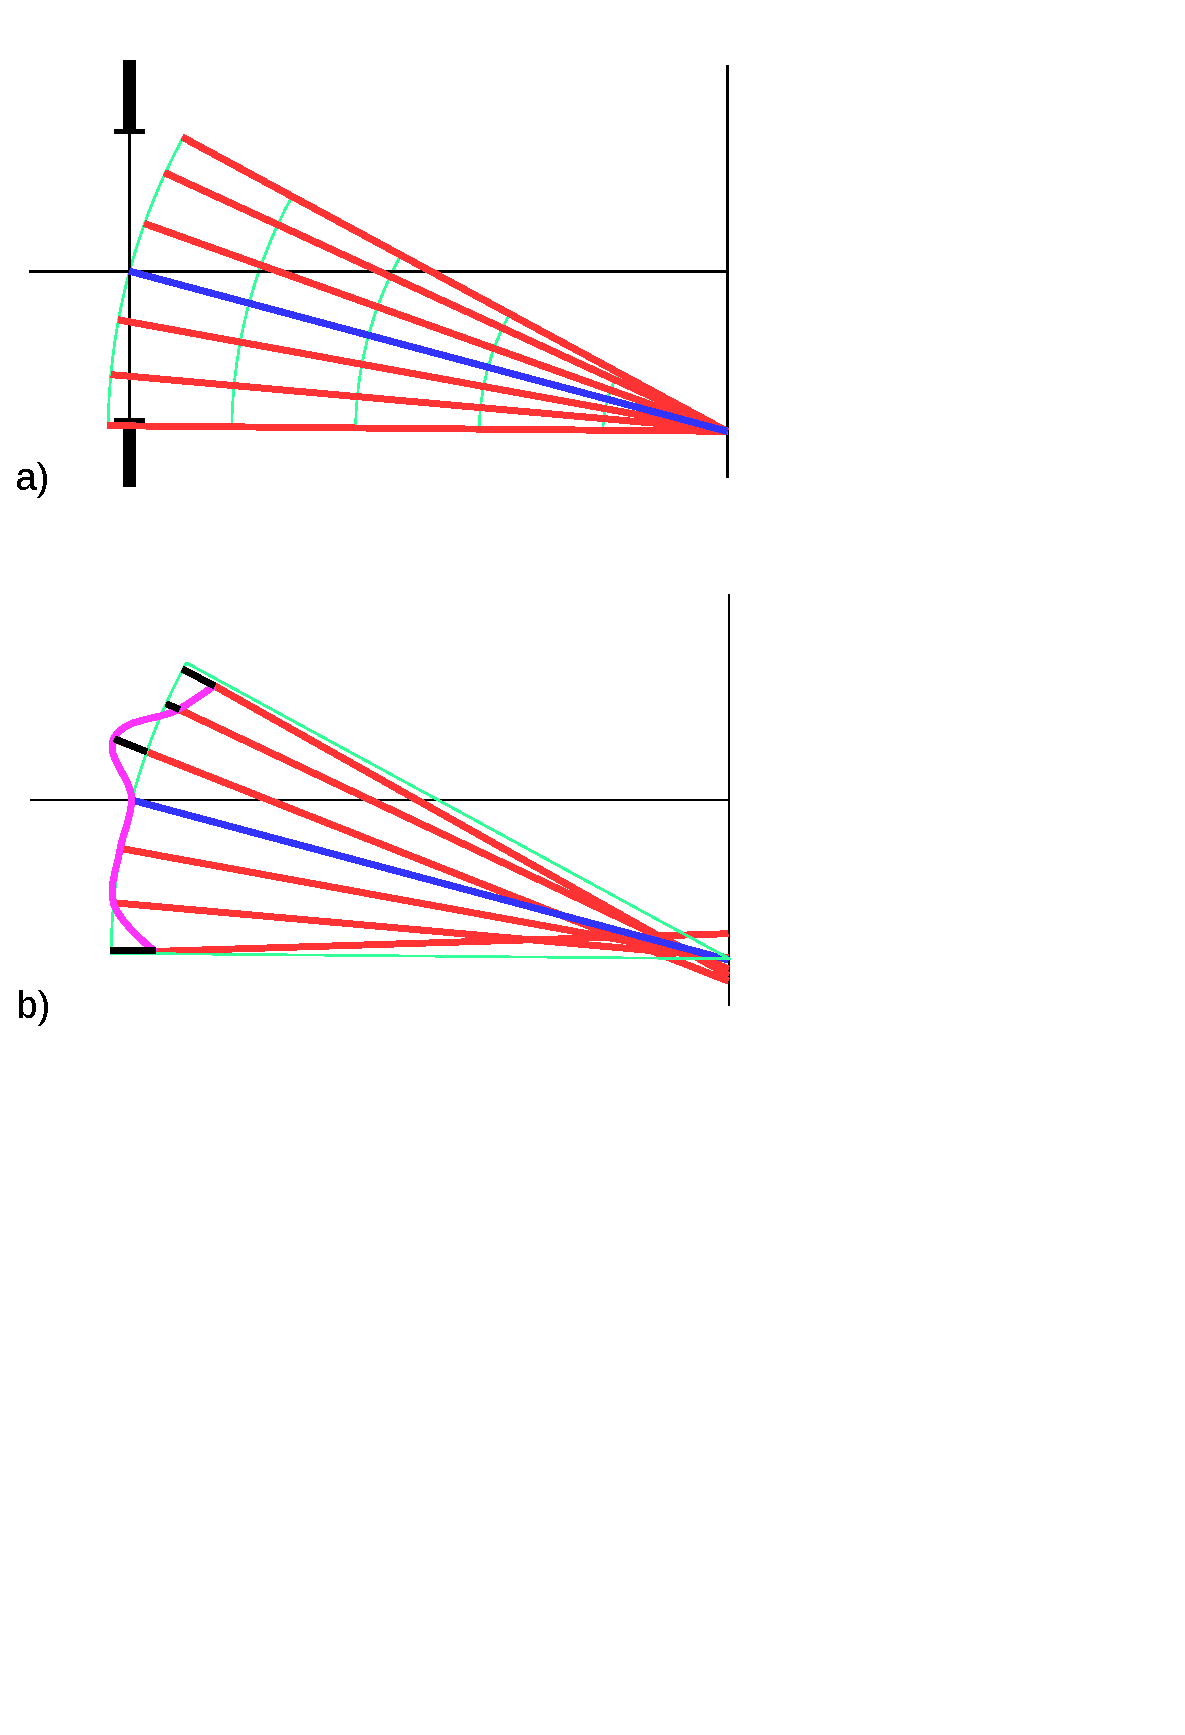
\includegraphics[width=0.5\columnwidth]{waveaberrations}\\ % waveaberrations file missing in tree!
  \caption{a) In a perfect system, according to the Fermat principle, all rays have the same time of flight from the object to the image. b) In a real system, wave aberrations occur. A line of constant time of flight is displayed in magenta.
  Wave aberrations are the optical path differences corresponding to the difference in time of flight when hitting the exit pupil reference sphere.}
  \label{fig:waveaberrations}
\end{figure}

\subsection{Calculation of wave aberrations}
TODO: this only works for on axis field points !!!

Assume we know the position $x_{im}, y_{im}$ and direction $\Vector{d}$ of a set of rays in the image plane and their geometric path length from the object to the image.
To obtain the wave aberrations, we intersect the rays with the spherical exit pupil.
The task is similar to the intersections performed throughout the raytracing, see section \ref{subsection:spheres}.
We center our coordinate system around the chief ray image position.

\begin{eqnarray}
 \Location &=& \begin{pmatrix} x_0 \\ y_0 \\ 0 \end{pmatrix} + \Vector{d} t \\
 \Location^2 &=& R^2
\end{eqnarray}
with
 \begin{eqnarray}
 \begin{pmatrix} x_0 \\ y_0 \end{pmatrix} &=& \begin{pmatrix} x_{im} \\ y_{im} \end{pmatrix} - \begin{pmatrix} x_{chief,im} \\ y_{chief,im} \end{pmatrix} \\
 z_{im} &=& 0 \\
 | \Vector{d} | &=& 1
\end{eqnarray}
Here, $R$ is the distance between exit pupil and image, and $t$ is the geometric path length of the back-propagation.

We find
\begin{eqnarray}
 R^2 &=&  t^2 + 2 (d_x x_0 + d_y y_0) t + x_0^2 + y_0^2 \\
 t_{1,2} &=& - (d_x x_0 + d_y y_0) \pm \sqrt{ (d_x x_0 + d_y y_0)^2 - (x_0^2 + y_0^2) + R^2 }
\end{eqnarray}

We assume that the macroscopic distance between image and exit pupil $R^2$ term under the root is much larger than the microscopic aberrations and use a Taylor expansion
\begin{eqnarray}
 t_{1,2} &\approx& R - (d_x x_0 + d_y y_0) \pm 
 \left[ 
   \frac{1}{2R} \delta - \frac{1}{8R^3} \delta^2
 \right]
 \\
 \delta &=& (d_x x_0 + d_y y_0)^2 - x_0^2 - y_0^2
\end{eqnarray}

The geometric path length $t$ is inserted into the material dispersion to obtain the retardation between exit pupil and image. After that, this propagation length is subtracted from the optical path length from object to image.
Another subtraction of the chief ray value normalizes the result.
By didviding with the vacuum wavelength, we obtain the wave aberration in number of waves.




\chapter{Appendix}

\section{Issues}

\begin{enumerate}
 \item minor: use private variables {\tt \underline{\;}\,\underline{\;}variable} and {\tt @property} and {\tt @variable.setter} getter and setter decorators to
      achieve a controled access to private variables but access them in a manner one would do for public variables (i.e. {\tt object.variable})
 \item Check for algorithms and formulas which are only valid in rotational symmetric systems
 \item Check for algorithms that are valid without immersion
 \item Optical system has to calculate absolute positions of its surfaces (including tilt) referenced to a given coordinate system.
 \item Optical system has to calculate relative coordinate transforms (translation, rotation) between certain elements
 \item Calculate coordinate transforms from ABCD/XYUV1 formalism
 \item Calculate XYUV1 matrices as generalization of ABCD
 \item Use some pilot ray (in optical axis system) for calculating (exact) intersection points at each surface, calculate local curvature at intersection point
      and calculate focal power in $x, y$. Calculate also tilt (and maybe decenter) of pilot ray at each surface. Combine both results as a matrix product in a resulting
      XYUV1 matrix
 \item Consider whether XYUV1 matrices should be 4x4, 5x5, 6x6, or 7x7.
 \item Raybundle.o array is referenced relative to the next surface vertex $\Rightarrow$ counter intuitive!
 \item Use absolute coordinates for 2D and 3D drawing procedures
 \item every class one file
 \item Plots of typical rayfans, wave aberration, Seidel coefficients, aberration plots vs pupil or field coordinates, PSF, image simulation, MTF, OTF
 \item ZMX import
 \item ZMX export
 \item GRIN (propagate function also for other materials)
 \item anisotropic media (uniaxial, biaxial)
 \item Pupil aiming for infinite object/image distance
 \item issue: getAllOptimizableVariables in opticalsystem?
 \item long term goal: investigate class structure to be simplified by design concepts of gang of four (Gamma, Helm, Johnson, Vlissides)
 \item long term goal: interface for freecad (systematically implement functionality)
 \item long term goal: Optimization: discrete for glass types, genetic/evolutionary algorithms
 \item long term goal: Image System data base and paraxial layout wizard
 \item long term goal: polarization
 \item long term goal: Fresnel coefficients, generalized for anisotropic media
\end{enumerate}

\section{Suggestions for linear and nonlinear transfer formalisms}
The following section shows some suggestions for linear and non-linear transfer formalisms
to simplify and unify ray tracing. The transfer formalisms should have the following properties:

\begin{itemize}
 \item They should be physical and not ad-hoc (physical foundations, quick access to conserved quantities and so on)
 \item A linear transfer formalism like $ABCD$ should be the linearisation of a non-linear transfer formalism
 \item They should be formulated with respect to the optical axis
 \item They should incorporate changes of the optical axis in a unified manner
\end{itemize}

\remark{It would be cool to only stich these transfer functions together like in the ABCD formalism;
this means in particular, that a ray just should move by $(\Vector{X}_f, \Vector{d}_f) = F_n (F_{n-1}( \dots F_2 (F_1(\Vector{X}_i, \Vector{d}_i))))$ where
the $F_k$ are functions discussed in the following subsections.}

\subsection{Nonlinear XYUV formalism}
According to {{\tt \url{http://graphics.stanford.edu/courses/cs148-10-summer/docs/2006--degreve--reflection_refraction.pdf}}}
we will call the incident vector $\Vector{i}$ the reflected one $\Vector{r}$ and the refracted one $\Vector{t}$.
From reflection law we get the following ($\Vector{n}$ is pointing into medium $n_1$ and the incidence vector is pointing from $n_1$ to $n_2$)
\begin{align}
 \Vector{r} &= \Vector{i} - 2 \scpm{\Vector{i}}{\Vector{n}} \Vector{n}\,.\label{eq:reflection_vector}
\end{align}
From refraction we get\remark{I know that is not as elegant as the former 
solution by considering the field components at material boundaries :-)}
\begin{align}
 \Vector{t} &= \frac{n_1}{n_2} \Vector{i} 
 - \left[\frac{n_1}{n_2} \scpm{\Vector{i}}{\Vector{n}} 
      + \sqrt{1 - \left(\frac{n_1}{n_2}\right)^2 (1 - {\scpm{\Vector{i}}{\Vector{n}}}^2)}\right] \Vector{n}\,.\label{eq:refraction_vector}
\end{align}
Let us now consider the optical axis $\Vector{e}_z$ and some starting point of the ray at distance $d_1$ at the left hand side
of the optical surface $F(x, y)$, $(x,y,-d_1)$. The direction vector is given by $\Vector{d} = (d_x, d_y, \sqrt{1 - d_x^2 - d_y^2})$.
The components of the direction vector are equivalent to some aiming angles. For our convenience we take our
four variables $(x, y, d_x, d_y)$ as free starting parameters and try to calculate the new parameters at distance $d_2$ behind the
optical surface $F(x, y)$, $(x', y', {d_x}', {d_y}')$, via some nonlinear transform $(x', y', {d_x}', {d_y}') = T(x, y, d_x, d_y)$,
where $T$ is some function $T:\mathbb{R}^4 \to \mathbb{R}^4$.

By using the formulas from \ref{subsec:intersectionformulas} it is possible to invert the equation 
\begin{align}
-d_1 + t \sqrt{1-d_x^2-d_y^2} &= F(x + t d_x, y + t d_y)\,,\label{eq:genintersection} 
\end{align}
for $t$ either analytically or numerically. The equation tells
us where the ray started at $x, y$, $z = -d_1$ intersects the surface $F(x, y)$. Let the solution
of this equation $t_\text{intersect} = \sigma(x, y, d_x, d_y)$. (Notice that the function $\sigma$
is in general nonlinear in its arguments, even for the simplest case of a sphere.) Then by using the 
sigma notation the intersection point is also given by a nonlinear vector entity:
\begin{align}
 \Vector{p}_\text{i} &= \begin{pmatrix} x + \sigma(x,y,d_x,d_y) d_x \\ y + \sigma(x,y,d_x,d_y) d_y \\ -d_1 + \sigma(x,y,d_x,d_y) \sqrt{1 - d_x^2 - d_y^2} \end{pmatrix}\,.\label{eq:pintersect}
\end{align}
The vector perpendicular on the surface pointing in direction of medium $n_1$ (left hand side, negative $z$ direction) is given
by
\begin{align}
 \Vector{n}(x, y) &= 
  \frac{1}{\sqrt{1 + (\Vector{\nabla}_{x,y} F)^2}} 
  \begin{pmatrix} \frac{\partial F}{\partial y} \\ \frac{\partial F}{\partial y} \\ -1 \end{pmatrix}\,.\label{eq:surfacenormal}
\end{align}
This vector has to be evaluated at $\Vector{p}_\text{i}$ to get the appropriate results for
the transmission and reflection direction. Now we may use \eqref{eq:refraction_vector} or \eqref{eq:reflection_vector}
and \eqref{eq:surfacenormal} evaluated at \eqref{eq:pintersect} to calculate the direction vector $\Vector{d}'(p_{\text{i} x}, p_{\text{i} y})$.
To calculate $x'$ and $y'$ we have to calculate another ray which starts at $p_\text{intersect}$ and ends at the
distance $d_2$ from the plane. Therefore $p_{\text{i}\,z} + t_\text{new} \sqrt{1 - {d'}_x^2 - {d'}_y^2} = d_2$ and so
\begin{align}
t_\text{new} &= \frac{d_2 - p_{\text{i}\,z}}{\sqrt{1 - {d'}_x^2 - {d'}_y^2}}\,.
\end{align}
Thus the final coordinates are given by
\begin{subequations}
\begin{align}
 x' &= p_{\text{i}\,x} + \frac{d_2 - p_{\text{i}\,z}}{\sqrt{1 - {d'}_x^2 - {d'}_y^2}} {d'}_x\,,\\
 y' &= p_{\text{i}\,y} + \frac{d_2 - p_{\text{i}\,z}}{\sqrt{1 - {d'}_x^2 - {d'}_y^2}} {d'}_y\,.
\end{align}
\end{subequations}
Collecting all together: The first $t$ value is (via inverting \eqref{eq:genintersection})
\begin{align}
 t_\text{intersect} &= \sigma(x, y, d_x, d_y) = \sigma\,.\label{eq:sigmasol}
\end{align}
The intersection point is given by
\begin{align}
 \Vector{p}_\text{i} &= \begin{pmatrix} x + \sigma d_x \\ y + \sigma d_y \\ -d_1 + \sigma \sqrt{1 - d_x^2 - d_y^2} \end{pmatrix}\,.
\end{align}
The unit normal vector has to be evaluated and according to \eqref{eq:surfacenormal} given by
\begin{align}
 \Vector{N} &:= \Vector{n}(p_{\text{i}x}, p_{\text{j}y})\,.\label{eq:surfacenormal2}
\end{align}
For a refractive problem the new direction vector is derived from \eqref{eq:refraction_vector} and therefore
\begin{align}
 \Vector{d}' &= \frac{n_1}{n_2} \Vector{d} 
 - \left[\frac{n_1}{n_2} \scpm{\Vector{d}}{\Vector{N}} 
      + \sqrt{1 - \left(\frac{n_1}{n_2}\right)^2 (1 - {\scpm{\Vector{d}}{\Vector{N}}}^2)}\right] \Vector{N}\,.\label{eq:newdirection}
\end{align}
and for the final coordinates after inserting the intersection point coordinates
\begin{subequations}
\label{eq:newposition}
\begin{align}
 x' &= x + \sigma d_x + \frac{d_2 + d_1 - \sigma \sqrt{1 - d_x^2 - d_y^2}}{\sqrt{1 - {d'}_x^2 - {d'}_y^2}} {d'}_x\,,\\
 y' &= y + \sigma d_y + \frac{d_2 + d_1 - \sigma \sqrt{1 - d_x^2 - d_y^2}}{\sqrt{1 - {d'}_x^2 - {d'}_y^2}} {d'}_y\,.
\end{align}
\end{subequations}
Eqns. \eqref{eq:newdirection} and \eqref{eq:newposition} together with \eqref{eq:surfacenormal2}, \eqref{eq:surfacenormal},
\eqref{eq:pintersect} and \eqref{eq:sigmasol} give the final nonlinear transformation for a refractive optical surface between
two materials with constant optical indices. Notice that $\sigma$ depends on the starting variables, too.  
For, e.g., a conic section it is given by (see \eqref{eq:intersectionconicsection})
\begin{align}
 \sigma_{\text{conic section}} &= \frac{G}{ F + \sqrt{F^2 + H G} }\,,
\end{align}
where
\begin{eqnarray}
   F &=& \sqrt{1 - d_x^2 - d_y^2} - \rho \left( d_x x + d_y y - d_1 (1+c) \sqrt{1 - d_x^2 - d_y^2} \right)\,, \\
   G &=& \rho (x^2 + y^2 + d_1^2 (1+c)) + 2 d_1\,, \\
   H &=& - \rho ( 1 + c \, (1 - d_x^2 - d_y^2) )\,.
\end{eqnarray}
In a strictly linear approximation of the new coordinates where we neglect all dependencies of $x$, $y$, $d_x$, $d_y$,
\begin{align}
 \sigma_\text{conic section} &\approx \frac{d_1}{1+ \frac{1}{\rho d_1 (1 + c)}} \stackrel{\rho d_1 (1+c)\gg 1}{\approx} d_1 \left(1 - d_1 \rho(1+c) + \mathcal{O}(\rho d_1 (1+c))^2\right)\,. 
\end{align}
If we further assume that we may neglect nonlinear terms in the new direction equation \eqref{eq:newdirection}
which means [we also approximate $\sigma \approx d_1$]\\
\begin{subequations}
 \begin{align}
  {d'}_x &= {\left(\left[\frac{n_{1}}{n_{2}} - 1\right]\rho \sigma + \frac{n_{1}}{n_{2}}\right)} d_{x} + {\left(\frac{n_{1}}{n_{2}} - 1\right)} \rho x\,,\\
  {d'}_y &= {\left(\left[\frac{n_{1}}{n_{2}} - 1\right]\rho \sigma + \frac{n_{1}}{n_{2}}\right)} d_{y} + {\left(\frac{n_{1}}{n_{2}} - 1\right)} \rho y\,,
 \end{align}
\end{subequations}
we can simplify the new coordinates to (note: linear approximation! So the square roots are $\approx1$!)
\begin{subequations}
\label{eq:linearapprox}
\begin{align}
 x' &\approx {\left({\left(\rho d_{1} \left(\frac{n_{1}}{n_{2}} - 1\right) + \frac{n_{1}}{n_{2}}\right)} d_{2} + d_{1}\right)} d_{x} + {\left(\rho d_{2} {\left(\frac{n_{1}}{n_{2}} - 1\right)} + 1\right)} x\,,\\
 y' &\approx {\left({\left(\rho d_{1} \left(\frac{n_{1}}{n_{2}} - 1\right) + \frac{n_{1}}{n_{2}}\right)} d_{2} + d_{1}\right)} d_{y} + {\left(\rho d_{2} {\left(\frac{n_{1}}{n_{2}} - 1\right)} + 1\right)} y\,.
\end{align}
\end{subequations}
Therefore the matrix formulation is given by
\begin{align}
 &\begin{pmatrix} x' \\ y' \\ {d'}_x \\ {d'}_y \end{pmatrix} =\nonumber\\ 
 &\begin{pmatrix} \rho d_{2} {\left(\frac{n_{1}}{n_{2}} - 1\right)} + 1 & 0 & {\left(\rho d_{1} \left(\frac{n_{1}}{n_{2}} - 1\right) + \frac{n_{1}}{n_{2}}\right)} d_{2} + d_{1} & 0 \\ 
		  0 & \rho d_{2} {\left(\frac{n_{1}}{n_{2}} - 1\right)} + 1 & 0 & {\left(\rho d_{1} \left(\frac{n_{1}}{n_{2}} - 1\right) + \frac{n_{1}}{n_{2}}\right)} d_{2} + d_{1} \\ 
		  \left(\frac{n_{1}}{n_{2}} - 1\right) \rho & 0 & \left[\frac{n_{1}}{n_{2}} - 1\right]\rho d_1 + \frac{n_{1}}{n_{2}} & 0 \\ 
		  0 & \left(\frac{n_{1}}{n_{2}} - 1\right) \rho & 0 & \left[\frac{n_{1}}{n_{2}} - 1\right]\rho d_1 + \frac{n_{1}}{n_{2}}\end{pmatrix}\nonumber\\ 
 &\times\begin{pmatrix} x \\ y \\ d_x \\ d_y \end{pmatrix}\,,
\end{align}
which is a very rough approximation.
This should be equivalent to translation by distance $d_1$ to the optical surface,
refraction of the rays at the optical surface (conic section) and translation by distance
$d_2$. Further we could reduce this problem to $ABCD$ matrices because there is no mixing
between $x$ and $y$ axis,
\begin{align}
 \begin{pmatrix} r'  \\ d' \end{pmatrix} &= 
 \begin{pmatrix} \rho d_{2} {\left(\frac{n_{1}}{n_{2}} - 1\right)} + 1 & {\left(\rho d_{1} \left(\frac{n_{1}}{n_{2}} - 1\right) + \frac{n_{1}}{n_{2}}\right)} d_{2} + d_{1} \\ 
		\left(\frac{n_{1}}{n_{2}} - 1\right) \rho &  \left[\frac{n_{1}}{n_{2}} - 1\right]\rho d_1 + \frac{n_{1}}{n_{2}} \end{pmatrix}
 \begin{pmatrix} r  \\ d \end{pmatrix}\,.
\end{align}
This is exactly the transformation which can be obtained from using the linear $ABCD$ matrix formalism by considering
\begin{align}
 \begin{pmatrix} r'  \\ d' \end{pmatrix} &=
 \begin{pmatrix} 1 & d_2 \\ 0 & 1 \end{pmatrix}
 \begin{pmatrix} 1 & 0 \\ \left(\frac{n_1}{n_2} - 1\right)\rho & \frac{n_1}{n_2} \end{pmatrix}
 \begin{pmatrix} 1 & d_1 \\ 0 & 1 \end{pmatrix}
 \begin{pmatrix} r  \\ d \end{pmatrix}\,.
\end{align}
Thus the linear approximation relies on the following points:
\begin{itemize}
 \item Small angles and small deviations from optical axis (linear approximation)
 \item Approximation of $\sigma$ by distance $d_1$ to surface 
 \item Linear approximation of normal vector of surface [this implies approximation of surface by local curvature at $x=y=0$]
 \item At least for the $ABCD$ formalism: rotationally symmetric surface
 \item Properties of surface enter the calculation only via $\sigma$ and $\Vector{N}$: the linear dependence of $\rho$ comes from $\Vector{N}$
\end{itemize}
\remark{Is it possible by comparison of fully nonlinear transfer formalism and linear approximation, i.e. $ABCD$ formalism, to obtain the
aberrations?}

\subsection{5x5 formalism}
In computer vision there are homogeneous coordinates used to implement translation and rotation in a single matrix.
There is a further coordinate $c$ introduced such that $\bar{x} = x/c, \bar{y} = y/c$ where $x$, $y$ and $c$
are the homogeneous coordinates and $\bar{x}$ and $\bar{y}$ are the view coordinates. Then general transformations have the following block
structure
\begin{align}
 \begin{pmatrix} \Vector{r}' \\ c' \end{pmatrix} &= 
 \begin{pmatrix}
  R & \Vector{t} \\
  0 & 1
 \end{pmatrix}
 \begin{pmatrix}
  \Vector{r} \\ 
  c
 \end{pmatrix}\,.
\end{align}
Therefore
\begin{align}
 \Vector{r}' &= R \Vector{r} + c \Vector{t}\,,\label{eq:homotransform}\\
 c' &= c
\end{align}
Usually one sets the $c$ equal to one and therefore $\Vector{r}'$ contains
the transformed coordinates already. As one can see in \eqref{eq:homotransform}
$\Vector{r}'$ is also translated.

In the $XYUV$ formalism $\Vector{r}$ and $\Vector{r}'$ are given by $(x,y,d_x,d_y)$ and $(x',y',{d'}_x,{d'}_y)$
respectively. To get a feeling for the transformation of the homogeneous coordinates we consider only
a translation
\begin{align}
 \begin{pmatrix} x' \\ y' \\ {d'}_x \\ {d'}_y \\ 1 \end{pmatrix} &=
 \begin{pmatrix} 1 & 0 & 0 & 0 & t_x \\
                 0 & 1 & 0 & 0 & t_y \\
                 0 & 0 & 1 & 0 & D_x \\
                 0 & 0 & 0 & 1 & D_y \\
                 0 & 0 & 0 & 0 & 1 \\
 \end{pmatrix}
 \begin{pmatrix} x \\ y \\ d_x \\ d_y \\ 1 \end{pmatrix}\,.
\end{align}
Therefore we get
\begin{subequations}
\begin{align}
 x' &= x + t_x\,,\\
 y' &= y + t_y\,,\\
 {d'}_x &= d_x + D_x\,,\\
 {d'}_y &= d_y + D_y\,.
\end{align}
\end{subequations}
which corresponds to a absolute change in intersection points and ray direction.
Notice that the new direction vector also has to be a unit vector such that
\begin{align}
 \underbrace{{\Vector{d}}^{\prime 2}}_{=1} &= \underbrace{\Vector{d}^2}_{=1} + 2 \scpm{\Vector{d}}{\Vector{D}} + \Vector{D}^2\,,
\end{align}
gives a condition to the third component of $\Vector{D}$, namely
\begin{align}
 D_z &= -\sqrt{1 - d_x^2 - d_y^2} \pm \sqrt{1 - (d_x + D_x)^2 - (d_y + D_y)^2}\,.
\end{align}
Maybe this extension of the $XYUV$ (non linear) transfer formalism can be useful as a further generalisation of
the optical design calculation. By multiplying the direction vector with the optical index one immediately gets
a so called phase space formulation of the optical ray. In this formulation several theorems from Hamiltonian
mechanics and phase space theory in general hold. These formulation will be investigated in further subsections.

\subsection{\texorpdfstring{$PQ$}{PQ}-2D-Formalism}

By using the equations of motion \eqref{eq:H2Deom} for appropriate materials one can write down non linear transfers for
some special materials.

\subsubsection{Nonlinear transfer formalism}

Transfer through homogeneous material:
\begin{align}
 \begin{pmatrix}
  \Vector{Q} \\
  \Vector{P}
 \end{pmatrix} &\mapsto
 \begin{pmatrix}
  \Vector{Q} + (z' -z) \frac{\Vector{P}}{n \sqrt{1 - \frac{\Vector{P}^2}{n^2}}} \\
  \Vector{P}
 \end{pmatrix}\,.
\end{align}
Here $H_{\text{2D}}$ stays constant because the 3D momentum is conserved.
According to Ibn-Sal-Snell's law the coordinate change at surface on surface $z = f(x,y)$ at $(\Vector{Q} , f(\Vector{Q}))$ is given by
\begin{align}
 &\begin{pmatrix}
  \Vector{Q} \\
  \Vector{P}
 \end{pmatrix} \mapsto\nonumber\\&
 \begin{pmatrix}
  \Vector{Q} \\
  \Vector{P} - \left[\scpm{\Vector{P}}{\Vector{N}(\Vector{Q})} + Z(\Vector{Q}) H + \sqrt{n_2^2 - n_1^2 + [\scpm{\Vector{P}}{\Vector{N}(\Vector{Q})} + Z(\Vector{Q})H]^2}\right] \Vector{N}(\Vector{Q})
 \end{pmatrix}\,,
\end{align}
where $H = -n_1 \sqrt{1 - \Vector{P}^2/n^2}$, 
$\Vector{N}(\Vector{Q}) = (\text{grad} f)(\Vector{Q})/\sqrt{1 + (\text{grad} f)^2(\Vector{Q})}$, 
$Z(\Vector{Q}) = 1/\sqrt{1 + (\text{grad} f)^2(\Vector{Q})}$.
For a complete optical system one has to perform this transformations in a succesive manner on the starting configuration of the ray.
Notice that due to the non-conservation of the Hamiltonian it will also change at the boundary between two layers in the following manner
\begin{align}
 H &\mapsto H + \left[\scpm{\Vector{P}}{\Vector{N}(\Vector{Q})} + Z(\Vector{Q}) H + \sqrt{n_2^2 - n_1^2 + [\scpm{\Vector{P}}{\Vector{N}(\Vector{Q})} + Z(\Vector{Q})H]^2}\right] Z(\Vector{Q})\,.
\end{align}



\subsubsection{Linear transfer formalism}

To get the paraxial approximation we need to expand the terms to linear order in $\Vector{P}$ (equivalent to a small angle approximation) and linear order in $\Vector{Q}$
(corresponding to near axis rays). An expansion only in $\Vector{Q}$ corresponds to near axis rays with finite angles and an $\Vector{P}$-only expansion corresponds to
small angle with finite field heights. The linearisation leads to a matrix formulation of the transfer functions.

For the transfer in a homogeneous material one gets
\begin{align}
 \begin{pmatrix}
  \Vector{Q} \\
  \Vector{P}
 \end{pmatrix} &\stackrel{\text{linear}}{\mapsto}
 \begin{pmatrix}
  \Vector{Q} + (z' -z) \frac{\Vector{P}}{n} \\
  \Vector{P}
 \end{pmatrix} =
 \begin{pmatrix}
  1 & \frac{z' - z}{n} \\
  0 & 1
 \end{pmatrix}
 \begin{pmatrix}
  \Vector{Q} \\
  \Vector{P}
 \end{pmatrix} 
\,.
\end{align}
For the refraction between two homogeneous materials $n_1$ and $n_2$ we get (Assume that the surface at $\Vector{Q}=0$ is not tilted and the surface
itself is a biconic with the two local curvatures in the respective coordinate directions $c_x$, $c_y$.)
\begin{align}
 \begin{pmatrix}
  \Vector{Q} \\
  \Vector{P}
 \end{pmatrix} &\stackrel{\text{linear}}{\mapsto}
 \begin{pmatrix}
  \Vector{Q} \\
  \Vector{P} + (n_1 - n_2) \begin{pmatrix} c_x & 0 \\ 0 & c_y \end{pmatrix}  \Vector{Q}
 \end{pmatrix} =
 \begin{pmatrix}
  1 & 0 & 0 & 0 \\
  0 & 1 & 0 & 0 \\
  (n_1 - n_2)c_x & 0 & 1 & 0   \\
  0 & (n_1 - n_2)c_y & 0 & 1  
 \end{pmatrix}
 \begin{pmatrix}
  \Vector{Q} \\
  \Vector{P}
 \end{pmatrix} 
\,.
\end{align}
Also the Hamitonian changes. This change is to first order in $\Vector{Q}$ and $\Vector{P}$ trivially
be given by
\begin{align}
 H_\text{2D} & \stackrel{\text{linear}}{\mapsto} -n_1 + (n_2 - n_1)\,.
\end{align}
But since a Hamiltonian in linear approximation is not sufficient to generate equations of motion,
one has to approximate at least to second order
\begin{align}
 \Delta H_\text{2D} &\stackrel{\text{quadratic}}{=} n_2-n_1
   +\frac{1}{2} \left(\frac{1}{n_1}-\frac{1}{n_2}\right) p_x^2
   + \frac{1}{2}  \left(\frac{1}{n_1}-\frac{1}{n_2}\right) p_y^2 \nonumber\\&
  -\frac{c_x^2 q_x^2 (n_1-n_2)^2}{2 n_2}+c_x p_x q_x \left(1-\frac{n_1}{n_2}\right)
   -\frac{c_y^2 q_y^2 (n_1-n_2)^2}{2 n_2}+c_y p_y q_y \left(1-\frac{n_1}{n_2}\right)
\,.
\end{align}


\subsection{\texorpdfstring{$pq$}{pq}-3D-Formalism}

The more general consideration of GRIN media in 3D phase space also fits into the formerly given transfer formalisms.
A ray starts at the point $(x,y,d_x,d_y)$ which means in a certain coordinate system
and a fixed $z$ position the ray starting point is $(x,y,z)$ and the direction vector
is $(d_x,d_y,\sqrt{1-d_x^2-d_y^2})$. This fixes the initial conditions of the ray propagation
uniquely. The 3D formulation is useful if the user parametrizes for another paramter then the distance $z$ on the optical
axis. In this case the Hamiltonian separates well in a kinetic and a potential term. Further the Hamiltonian is conserved and
equal zero.

\subsubsection{Nonlinear transfer}

Transfer through homogeneous medium to arc length $s$
\begin{align}
 \begin{pmatrix}
  \Vector{q} \\
  \Vector{p}
 \end{pmatrix} &\mapsto
 \begin{pmatrix}
  \Vector{q} + s \frac{\Vector{p}}{n} \\
  \Vector{p}
 \end{pmatrix}\,.
\end{align}
Notice that this transformation is not nonlinear.
Refraction at optical surface $f(x,y)$.
\begin{align}
 \begin{pmatrix}
  \Vector{q} \\
  \Vector{p}
 \end{pmatrix} &\mapsto
 \begin{pmatrix}
  \Vector{q} \\
  \Vector{p} - \left[\scpm{\Vector{p}}{\Vector{n}(\Vector{q})} + \sqrt{n_2^2 - n_1^2 + \scpm{\Vector{p}}{\Vector{n}(\Vector{q})}^2}\right] \Vector{n}(\Vector{q})
 \end{pmatrix}\,.
\end{align}
Notice that the Hamiltonian $H_\text{3D} = \Vector{p}^2 - n^2 = 0$ is conserved.
GRIN-Medium:
\begin{align}
 \begin{pmatrix}
  \Vector{q} \\
  \Vector{p}
 \end{pmatrix} &\stackrel{\text{ODE solver}}{\mapsto}
 \begin{pmatrix}
  \Vector{q}(s) \\
  \Vector{p}(s)
 \end{pmatrix}\,.
\end{align}


\subsubsection{Linearized transfer}
Only for refraction (this time also with tilted surface, where $\Vector{n}_0 = \Vector{n}(0)$ is the surface tilt vector):
\begin{align}
 \begin{pmatrix}
  \Vector{q} \\
  \Vector{p}
 \end{pmatrix} &\stackrel{\text{linear}}{\mapsto}
 \begin{pmatrix}
  \Vector{q} \\
  -\sqrt{n_2^2 - n_1^2} \Vector{n}_0 + \Vector{p} - \scpm{\Vector{p}}{\Vector{n}_0} \Vector{n}_0 - \sqrt{n_2^2 - n_1^2} [\scpm{\Vector{q}}{\Vector{\nabla}} \Vector{n}]_0
 \end{pmatrix}\nonumber\\&=
 \begin{pmatrix}
  1 & 0\\
  -\sqrt{n_2^2-n_1^2} (\Vector{\nabla} \otimes \Vector{n})_0 & 1 - \Vector{n}_0 \otimes \Vector{n}_0
 \end{pmatrix}
 \begin{pmatrix}
  \Vector{q} \\
  \Vector{p}
 \end{pmatrix} -
 \begin{pmatrix}
  0 \\
  \sqrt{n_2^2-n_1^2} \Vector{n}_0
 \end{pmatrix}
\,.
\end{align}
The absolute term which arises due to surface tilt may be absorbed into a homogenious formulation by using the 5x5 formalism mentioned above.

\subsection{Combined 2D 5x5 formalism}

We will start at a nonlinear homogeneous matrix transfer function of 3D variables and try to implement the formalisms discussed above
\begin{align}
 \begin{pmatrix}
  \Vector{q}\,{}'\\
  \Vector{p}\,{}'\\
  1
 \end{pmatrix}
 &=
 \underbrace{\begin{pmatrix}
  A(\Vector{q},\Vector{p}) & B(\Vector{q},\Vector{p}) & \Vector{t}(\Vector{q},\Vector{p})\\
  C(\Vector{q},\Vector{p}) & D(\Vector{q},\Vector{p}) & \Vector{\delta}(\Vector{q},\Vector{p})\\
  0 & 0 & 1 
 \end{pmatrix}}_\mathcal{T}
 \begin{pmatrix}
  \Vector{q}\\
  \Vector{p}\\
  1
 \end{pmatrix}\,.
\end{align}
As already discussed above this homogeneous transformation is able to include rotation and translation of the optical axis (aka coordinate breaks) 
in a unified manner. Due to the nonlinearity the formulation of the transfer matrix is not unique. Notice that the components of $\Vector{p}$ and $\Vector{p}\,{}'$
are not fully independent from each other. For unification with 2D formalism we split up the canonical coordinates and momenta into 2D and 3-components, i.e.
$\Vector{q} = (\Vector{Q}, z) = (Q_\alpha, z)$ where indices from the beginning of the greek alphabet are running over $1,2$. Now we also use Einstein summation
convention. Therefore the equation $\Vector{q}\,{}' = A \Vector{q}$ is $(2+1)$ decomposed like the following
\begin{align}
 Q^\prime_\alpha &= A_{\alpha\beta} Q_\beta + A_{\alpha 3} z\,,\\
 z^\prime &= A_{3 \beta} Q_\beta + A_{33} z\,.
\end{align}
For the readers convenience we omit the $(\Vector{q},\Vector{p})$ dependency of the sub matrices and vectors in the large transfer matrix.
In its full form the transfer reads (notice $H$ and $H'$ are the respective 2D Hamiltonians corresponding to the negative 3-component of the 2D momentum)
\begin{subequations}
\label{eq:transfermatrixeqns}
\begin{align}
 Q^\prime_\alpha &= A_{\alpha\beta} Q_\beta + A_{\alpha 3} z + B_{\alpha\beta} P_\beta - B_{\alpha 3} H + t_\alpha\,,\\
 z^\prime &= A_{3 \beta} Q_\beta + A_{33} z + B_{3\beta} P_\beta - B_{33} H + t_3\,,\\
 P^\prime_\alpha &= C_{\alpha\beta} Q_\beta + C_{\alpha 3} z + D_{\alpha\beta} P_\beta - D_{\alpha 3} H + \delta_\alpha\,,\\
 H' &= -C_{3\beta} Q_\beta - C_{33} z - D_{3\beta} P_\beta + D_{33} H - \delta_3\,,
\end{align}
\end{subequations}
Notice that the transfer function in this form is only valid for non-GRIN media. I would suggest to treat the transfer function of a GRIN medium
like a box where you put in $Q_\alpha, P_\alpha, z$ and after the propagation to $z'$ it spits out the primed coordinates.
\subsubsection{Transfer matrix functions}
For transfer through material with constant optical index $n$ we have
\begin{align}
 \begin{pmatrix}
  \Vector{Q} \\
  \Vector{P}
 \end{pmatrix} &\mapsto
 \begin{pmatrix}
  \Vector{Q} + (z' -z) \frac{\Vector{P}}{n \sqrt{1 - \frac{\Vector{P}^2}{n^2}}} \\
  \Vector{P}
 \end{pmatrix}\,.
\end{align}
So \eqref{eq:transfermatrixeqns} gives
\begin{align}
 A_{\alpha\beta} &= \delta_{\alpha\beta}\,,\quad A_{\alpha 3} = 0\,,\quad B_{\alpha\beta} = \frac{L}{\sqrt{n^2 - \Vector{P}^2}} \delta_{\alpha\beta}\,,\quad B_{\alpha3} = 0\,,\quad t_\alpha = 0 \\
 A_{3\beta} &= 0\,,\quad A_{33} = 1\,,\quad B_{3\beta} = 0\,,\quad B_{33} = 0\,,\quad t_3 = L\,,\\
 D_{\alpha\beta} &= \delta_{\alpha\beta}\,,\quad D_{33} = 1\,,
\end{align}
all other zero. Therefore\remark{check!}
\begin{align}
 \mathcal{T}_n &=
 \begin{pmatrix}
  \delta_{\alpha\beta} & 0 &  \frac{L}{\sqrt{n^2 - \Vector{P}^2}} \delta_{\alpha\beta} & 0 & 0\\
   0                   & 1 & 0 & 0 & L\\
   0                   & 0 & \delta_{\alpha\beta} & 0 & 0\\
   0                   & 0 & 0 & 1 & 0 \\
   0 & 0 & 0 & 0 & 1
 \end{pmatrix}
\end{align}
For refraction\remark{check!}
\begin{align}
 \mathcal{T}_{n_1\mapsto n_2} &=
 \begin{pmatrix}
  \delta_{\alpha\beta} & 0 &  0 & 0 & 0\\
   0                   & 1 & 0 & 0 & 0\\
   0                   & 0 & \delta_{\alpha\beta} & Z(\Vector{Q}) N_\alpha & -\biggl[\scpm{\Vector{P}}{\Vector{N}} - \sqrt{n_2^2 - n_1^2 + (\scpm{\Vector{P}}{\Vector{N}} + Z(\Vector{Q}) H)^2}\biggr] N_\alpha \\
   0                   & 0 & 0 & 1 + Z(\Vector{Q})^2 & -\biggl[\scpm{\Vector{P}}{\Vector{N}} - \sqrt{n_2^2 - n_1^2 + (\scpm{\Vector{P}}{\Vector{N}} + Z(\Vector{Q}) H)^2}\biggr] Z(\Vector{Q}) \\
   0 & 0 & 0 & 0 & 1
 \end{pmatrix}
\end{align}
For reflection\remark{check!}
\begin{align}
 \mathcal{T}_{\text{mirror}} &=
 \begin{pmatrix}
  \delta_{\alpha\beta} & 0 &  0 & 0 & 0\\
   0                   & 1 & 0 & 0 & 0\\
   0                   & 0 & \delta_{\alpha\beta} & 2 Z(\Vector{Q}) N_\alpha(\Vector{Q}) & -2 \scpm{\Vector{P}}{\Vector{N}} N_\alpha(\Vector{Q}) \\
   0                   & 0 & 0 & 1 - 2 Z(\Vector{Q})^2 & 2 \scpm{\Vector{P}}{\Vector{N}} Z(\Vector{Q}) \\
   0 & 0 & 0 & 0 & 1
 \end{pmatrix}
\end{align}
Notice that for a proper treatment of refraction or reflection at a curved surface one has to start a ray in the reference plane of the 
optical surface and propagate up to the surface. The intersection calculation is not trivial and only for special cases
available in closed form. After this intersection calculation one may calculate the normal vector at the intersection point
and refract the ray.

For coordinate break (rotation of momentum direction)
\begin{align}
 \mathcal{T}_{\text{CB,pR}} &=
 \begin{pmatrix}
  \delta_{\alpha\beta} & 0 &  0 & 0 & 0\\
   0                   & 1 & 0 & 0 & 0\\
   0                   & 0 & R_{\alpha\beta} & R_{\alpha 3} & 0 \\
   0                   & 0 & R_{3\beta} & R_{33} & 0 \\
   0 & 0 & 0 & 0 & 1
 \end{pmatrix}
\end{align}
For coordinate break (translation of intersection point)
\begin{align}
 \mathcal{T}_{\text{CB,T}} &=
 \begin{pmatrix}
  \delta_{\alpha\beta} & 0 &  0 & 0 & t_\alpha\\
   0                   & 1 & 0 & 0 & t_3\\
   0                   & 0 & \delta_{\alpha\beta} & 0 & 0 \\
   0                   & 0 & 0 & 1 & 0 \\
   0 & 0 & 0 & 0 & 1
 \end{pmatrix}
\end{align}
For coordinate break (rotation of intersection point inplane)
\begin{align}
 \mathcal{T}_{\text{CB,QR}} &=
 \begin{pmatrix}
  R_{\alpha\beta} & 0 &  0 & 0 & 0\\
   0                   & 1 & 0 & 0 & 0\\
   0                   & 0 & \delta_{\alpha\beta} & 0 & 0 \\
   0                   & 0 & 0 & 1 & 0 \\
   0 & 0 & 0 & 0 & 1
 \end{pmatrix}
\end{align}
These transformations can be combined in a matrix manner since they
are linear and have no dependency from the coordinates and momentum variables.
The nonlinear transfer functions could also be combined in a matrix manner but
one has to take care about the right arguments to the components.


\subsubsection{Linearisation}

For a linearized theory one has to treat the coordinate part ($A$, $B$, $C$, $D$) in a different manner than the absolute part ($\Vector{t}$, $\Vector{\delta}$).
The former has to be approximated only to zeroth order since they are multiplied by momenta and coordinates. In contrast the latter one
has to be approximated at first order to generate missing linear terms. Therefore the structure of the linearized theory can still change, but
at least there is a unique formalism to derive the paraxial approximation.
\begin{align}
  \mathcal{T} &= \begin{pmatrix}
  A_{ab}(\Vector{q},\Vector{p}) & B_{ab}(\Vector{q},\Vector{p}) & t_{a}(\Vector{q},\Vector{p})\\
  C_{ab}(\Vector{q},\Vector{p}) & D_{ab}(\Vector{q},\Vector{p}) & \delta_{a}(\Vector{q},\Vector{p})\\
  0 & 0 & 1 
 \end{pmatrix}
 \approx \nonumber\\&
  \begin{pmatrix}
  A(0,0) & B(0,0) & t_a(0,0) + (\partial^q_b t_a)(0,0) q_b + (\partial^p_b t_a)(0,0) p_b\\
  C(0,0) & D(0,0) & \delta_a(0,0) + (\partial^q_b \delta_a)(0,0) q_b + (\partial^p_b \delta_a)(0,0) p_b\\
  0 & 0 & 1 
 \end{pmatrix} \nonumber\\&
  \begin{pmatrix}
  A_{ab}(0,0)  + (\partial^q_b t_a)(0,0) & B_{ab}(0,0)+ (\partial^p_b t_a)(0,0) & t_a(0,0) \\
  C_{ab}(0,0)+ (\partial^q_b \delta_a)(0,0) & D_{ab}(0,0)  + (\partial^p_b \delta_a)(0,0)& \delta_a(0,0)\\
  0 & 0 & 1 
 \end{pmatrix}
\end{align}
After a ($2+1$) decomposition it is clear how to transform the 2D components of momentum and coordinates. (Notice
as mentioned earlier for the Hamiltonian, i.e. the negative 3-component of the momentum, it is not sufficient
to approximate to first order to generate the appropriate equations of motion. This means the $C_3$ and $D_3$ components
have to approximated at least to first order and the $\delta_3$ component up to second order.) Simple propagation in 2D is already linear.

Refraction:
\begin{align}
  \mathcal{T}_{n_1\mapsto n_2} \approx \begin{pmatrix}
  \delta_{ab} & 0 & 0 \\
   -\sqrt{n_2^2 - n_1^2} (\partial_b n_a)(0) & \delta_{ab} - n_a(0) n_b(0)& -\sqrt{n_2^2 - n_1^2} n_a(0)\\
  0 & 0 & 1 
 \end{pmatrix}
\end{align}
The first term second row depends on the curvature of the surface in the different directions. The second term is
a projection operator perpendicular to the unit normal vector of the surface at the optical axis.

Reflection:
\begin{align}
  \mathcal{T}_{\text{mirror}} \approx \begin{pmatrix}
  \delta_{ab} & 0 & 0 \\
   0 & \delta_{ab} - 2 n_a(0) n_b(0)& 0\\
  0 & 0 & 1 
 \end{pmatrix}
\end{align}
The higher order corrections in the taylor expansion give rise to the aberrations.

\subsection{Linearisation for non-zero interaction point with optical axis}
\newcommand{\dqv}{\Delta \Vector{q}}
\newcommand{\dpv}{\Delta \Vector{p}}

\newcommand{\dqi}[1]{\Delta q_{#1}}
\newcommand{\dpi}[1]{\Delta p_{#1}}


\newcommand{\qnv}{\Vector{q}_0}
\newcommand{\pnv}{\Vector{p}_0}

\newcommand{\qni}[1]{q_{0\,#1}}
\newcommand{\pni}[1]{p_{0\,#1}}
Let the optical axis at a certain surface start at $\Vector{q}_0$ and $\Vector{p}_0$ then (in 3D formalism)
the matrix deviation from it in linear approximation is given by
\begin{align}
  \mathcal{T} &= 
 \begin{pmatrix}
  A_{ab}(\qnv + \dqv,\pnv + \dpv) & B_{ab}(\qnv + \dqv,\pnv + \dpv) & t_{a}(\qnv + \dqv,\pnv + \dpv)\\
  C_{ab}(\qnv + \dqv,\pnv + \dpv) & D_{ab}(\qnv + \dqv,\pnv + \dpv) & \delta_{a}(\qnv + \dqv,\pnv + \dpv)\\
  0 & 0 & 1 
 \end{pmatrix}
\end{align}
A complete transformation is therefore split up into two parts
\begin{align}
 \begin{pmatrix}
  \qnv^\prime + \dqv^\prime\\
  \pnv^\prime + \dpv^\prime\\
  1
 \end{pmatrix} &=
  \mathcal{T}_{0} 
 \begin{pmatrix}
  \qnv \\
  \pnv \\
  1
 \end{pmatrix} +
  \Delta \mathcal{T}
 \begin{pmatrix}
  \dqv \\
  \dpv \\
  1
 \end{pmatrix}\,.
\end{align}
$\mathcal{T}_0$ is depending only on $\qnv$ and $\pnv$. It is obviously given by
\begin{align}
 \mathcal{T}_0 &= 
 \begin{pmatrix}
  A_{ab}(\qnv,\pnv) & B_{ab}(\qnv,\pnv) & t_{a}(\qnv,\pnv)\\
  C_{ab}(\qnv,\pnv) & D_{ab}(\qnv,\pnv) & \delta_{a}(\qnv,\pnv)\\
  0 & 0 & 1 
 \end{pmatrix}
\end{align}
This is the part transforming the optical axis or some kind of reference ray. The second part $\Delta \mathcal{T}$ comes from the transformation
of the linear deviation components with respect to the optical axis or the reference ray.
\begin{align}
 &\Delta \mathcal{T} = \nonumber\\&
 \begin{pmatrix}
  A_{ab} |_{0}+ \partial^q_b A_{ac}|_{0} \qni{c}  + \partial^q_b B_{ac} |_{0} \pni{c} + \partial^q_b t_a |_{0} &
   B_{ab} |_0 +  \partial^p_b A_{ac} |_{0} \qni{c} + \partial^p_b B_{ac} |_0 \pni{c} + \partial^p_b t_a |_0 & 0\\
  C_{ab} |_{0} + \partial^q_b C_{ac}|_{0} \qni{c} + \partial^q_b D_{ac} |_{0} \pni{c} + \partial^q_b \delta_a |_{0} &
   D_{ab} |_0 + \partial^p_b C_{ac} |_{0} \qni{c} + \partial^p_b D_{ac} |_0 \pni{c} + \partial^p_b \delta_a |_0 & 0\\
  0 & 0 & 0 
 \end{pmatrix}
\end{align}
Due to this split one may transform the optical axis in a first step and afterwards calculate the ``paraxial approximation'' of rays which
only deviate a little from the optical axis. All quantities have to be evaluated at the coordinates of the optical axis. The first terms
in the transfer matrix are the same as for the optical axis. All other terms (the derivatives) represent the deviations from it.
For an appropriate 5x5 treatment one has to decompose the matrix components further in a 2+1 manner.


\end{document}
